
%========= File containing the main LaTex document ========%
%                                                          %
% Copyright (C) ISI - All Rights Reserved                  %
% Proprietary                                              %
% Written by Med Hossam <med.hossam@gmail.com>, April 2016 %
%                                                          %
% @author: HEDHILI Med Houssemeddine                       %
% @linkedin: http://tn.linkedin.com/in/medhossam           %
%==========================================================%

%\documentclass[pfe]{./tpl/isipfe}

\newcommand{\Introduction}[1]{%
  \chapter*{#1}
  \addcontentsline{toc}{chapter}{#1}
}
\documentclass[]{./tpl/pfe}
\usepackage{longtable}
\usepackage{fancyhdr}
\usepackage{ctable}
\usepackage{colortbl}
\usepackage{geometry}
\usepackage{float}
\usepackage{wrapfig}
%\usepackage{hyperref}
% @author: front
% the command `\makeindex` is mandatory to create the index file main.idx
% https://tex.stackexchange.com/questions/9913/input-index-file-not-found
\makeindex

\begin{document}
    %
%=== File containing Global Configuration of the report ===%
%                                                          %
% Copyright (C) ISI - All Rights Reserved                  %
% Proprietary                                              %
% Written by Med Hossam <med.hossam@gmail.com>, April 2016 %
%                                                          %
% @author: HEDHILI Med Houssemeddine                       %
% @linkedin: http://tn.linkedin.com/in/medhossam           %
%==========================================================%

%=========== You MUST type your information here ==========%
% global_config.tex file is designed to configure your     %
% cover pages (main, back and black covers)                %
%==========================================================%

%============= Config new columns type ==============%
\newcolumntype{L}{>{\raggedright\arraybackslash}}
\newcolumntype{R}{>{\raggedleft\arraybackslash}}
\newcolumntype{C}{>{\centering\arraybackslash}}
%==================================================%

%========= Config the cover section ==========%

\title{Titre du projet}

\author{Prénom NOM}
%%% if necessary
% Set isBinomal to true and type second author name
%\setboolean{isBinomal}{true}
%\secondAuthor{Prénom NOM}

\diplomaName{Diplôme National d'Ingénieur en Sciences Appliquées et Technologiques}
\speciality{Génie Logiciel et Systèmes d'Information}
%\speciality{Génie des Télécommunications et Réseaux}
%\speciality{Génie Informatique des Systèmes Industriels}

%% Encadrant professionnel
\proFramerName{Monsieur/Madame Prénom NOM}
\proFramerSpeciality{Ingénieur R\&D}

%% Encadrant académique
\academicFramerName{Monsieur/Madame Prénom NOM}
\academicFramerSpeciality{Maître Assistant(e)}

%% Entreprise d'accueil
\companyName{Tunisie Télécome}

%% Année universitaire
\collegeYear{2017 - 2018}

%%%%%% Signatures section %%%%%%

% You can simply remove theses sentences by typing an empty string
% \proSignSentence{}

\proSignSentence{J'autorise l'étudiante à faire le dépôt de son rapport de stage en vue d'une soutenance.}

\academicSignSentence{J'autorise l'étudiante à faire le dépôt de son rapport de stage en vue d'une soutenance.}

%%% AR
\arabicAbstract{كجزء من تدريبنا الصيفي ، كانت مهمتنا هي تصميم وتطوير نموذج مولد في شكل دليل على المفهوم. سيتيح لنا هذا التطبيق إنشاء نماذج مخصصة ومصممة بشكل جيد وجاهزة للاندماج في تطبيقات الويب...}

\arabicAbstractKeywords{إثبات المفهوم ، مولد النموذج}

%% To use latin characters inside the arabic text
% just put them inside the command \textLR{}
%%%%

%%% FR
\frenchAbstract{Dans le cadre de notre stage d'été, nous avons eu comme mission la conception et le développement d'un générateur formulaire sous forme d'un POC. Cette application nous permettera de générer rapidement des formulaires bien conçus, personnalisé et prêts à être intégrés dans les applications web.}

\frenchAbstractKeywords{ Preuve de concept, Générateur Formulaire }

%%% EN
\englishAbstract{As part of our summer internship, our mission was to design and develop a form generator in the form of a POC. This application will allow us to quickly generate well-designed, personalized forms ready to be integrated into web applications.}

\englishAbstractKeywords{Proof of concept, Form Generator}

%% if you want to get rid of the company address just set the boolean variable to false
% PS : it's optional
\setboolean{wantToTypeCompanyAddress}{false}

\companyEmail{contact@company.com}
\companyTel{71 190 195}
\companyFax{71 222 222}
\companyAddressAR{نهج بحيرة ملاران - ضفاف البحيرة - تونس}
\companyAddressFR{Immeuble HERTZ, Borj Louizir, Ariana}
    
    \frontmatter
       %\addtolength{\topmargin}{-.875in}
\newgeometry{top=0.8cm,bottom=0.8cm,left=1cm,right=1cm}

\begin{titlepage}
{
\noindent Réf: ..../.......{\hfill 
         \hfill}\hfill AU: 2017-2018
\begin{center}
\vspace{-1cm}
\Huge \bfseries Université de Sousse
\setlength{\arrayrulewidth}{.2em}
\bigskip
\begin{tabular}{ccccccccccccccccccccccc}
\arrayrulecolor{blue}
\hline
\Huge \bfseries Ecole Nationale d’Ingénieurs de Sousse
\end{tabular}
\vspace{-1cm}
\begin{figure} [H]
    \centering
         \begin{center}
           
\includegraphics[scale=0.1]{img/Logo_ENISo.png}
        \end{center}
\end{figure}
\vspace{-1.2cm}
\textsc{\LARGE Rapport de Stage-ingénieur}\\
\textsc{\large Sujet:}\\
\textsc{\Huge Générateur de formulaires}\\
\textsc{\large Réalisé par :}\\
\vspace{-0.9cm}
\textsc{\LARGE Nesrine Sghaier}\\
\textsc{\large Filière :}\\
\vspace{-0.8cm}
\textsc{\LARGE 2ème  Année  Génie Informatique Appliquée}\\
\textsc{\large Stage effectué au sein de la Société:}\\
\textsc{\Huge Sofia HOLDINGS}\\
\begin{figure} [H]
    \centering
         \begin{center}
           
\includegraphics[scale=0.6]{img/sofia-technologies.jpg}
        \end{center}
\end{figure}
\vspace{-1cm}
\textsc{\large adresse: Rue des Entrepreneurs, Charguia 2} 

\end{center}
\bigskip
\noindent             {\hfill 
         \hfill}\hfill Période du stage : 03/07/2018 - 31/08/2018
}
\end{titlepage}


        \restoregeometry
\chapter*{\huge Remerciements}
%\addtolength{\topmargin}{0.5in}

\begin{center}
\it \Large
Je dédie ce travail à tous ceux qui me sont chers et particulièrement : \\

A mes Parents\\
Pour leur amour, leur patience et leur générosité, pour tous les efforts qu’ils ont consentis en ma faveur. J’espère avoir été digne de leur affection et de leur confiance.\\
A tous mes chers amis\\
Je leur dois une profonde reconnaissance et je vous assure de mes sincères sentiments
\end{center}

        
        \setcounter{page}{1}
        \setcounter{secnumdepth}{2}
        \setcounter{tocdepth}{2}
        \dominitoc
        \tableofcontents
        \adjustmtc
        \thispagestyle{frontmatter}
        \listoffigures
        \thispagestyle{frontmatter}
        \listoftables
        \thispagestyle{frontmatter}
        
       % \section*{Introduction générale}
%\section*{Introduction}
\addcontentsline{toc}{section}{Introduction générale}
%\markboth{Introduction générale}{} %To redefine the section page head
Un Formulaire est un très bon moyen de recueillir des données qui seront par la suite exploitables dans une multitude de cas: améliorer l’expérience utilisateur sur les sites, améliorer les produits et les services, avoir de nouvelles idées ...
La réalisation d'un tel questionnaire en ligne n'était pas toujours une chose aisée, avec le développement d’Internet, de nombreux outils ont vu le jour. Il existe à l’heure actuelle un grand nombre de logiciels de création de questionnaires en ligne mais chacun répondra à des attentes différentes.\\

Afin de répondre à des besoins précis et personnaliser ces outils informatiques d'une manière plus efficace pour l’amélioration au niveau de la qualité de ses services, l'entreprise SOFIA Technologies a proposé dans le cadre de ce projet la réalisation d'une application web qui permet de générer des formulaires dynamiques en ligne.\\    

Notre travail se traduit dans ce rapport qui développe les différentes phases par lesquelles nous sommes passées et qui sont organisées en trois chapitres de la manière suivante: \\
Nous débutons par présenter le cadre du projet, l’étude et la critique de l’existant, les objectifs
à atteindre, le langage et la méthodologie adoptés.\\
Le deuxième chapitre sera consacré à l’analyse et l’étude des besoins au cours duquel nous
allons énumérer les besoins fonctionnels et non fonctionnels, les intervenants au sein de notre
système et la conception de notre application.\\
La réalisation des sprints sera effectuée au niveau du dernier chapitre durant lequel nous allons détailler les différentes
fonctionnalités de l'application et les outils et les technologies utilisés.\\

Nous clôturerons ce rapport par une conclusion générale dans laquelle nous évaluerons le
travail réalisé au sein de la société et nous proposerons des perspectives dans le but d’améliorer
notre travail.

    %    \thispagestyle{frontmatter}
    
    \mainmatter
        \addcontentsline{toc}{chapter}{Fiche-synthèse du stage}
\thispagestyle{empty}

\begin{center}
    \begin{table}[!ht]
    \center
   \begin{tabular}{| p{6cm} | p{8cm}|}
\hline
\textbf {Nom d l’entreprise }  & Sofia Technologies \\ \hline
\textbf{Ville } & Charguia2, Ariana \\ \hline
\textbf{Nom de l’encadrant industriel} & Mokhles Ben Amor\\ \hline
\textbf{Date début et date fin du stage} & 02/07/2018 à 31/08/2018\\ 
\hline
\textbf{Nombre de jours effectifs passés dans les locaux de l’entreprise} & 50 jours \\ 
\hline
\textbf{Les  principales tâches réalisées durant le stage (maximum 3)} & - conception de l'application web du stage
\newline
- développement de application du stage 
\newline
- phase de test\\
\hline
\textbf{Le stage contient-il une période d’observation ?  si oui combien de jours ça a durée.} & non\\ 
\hline
\textbf{Le stage contient-il une partie conception ?  si oui combien de jours ça a pris} & oui, cela en une durée de 10 jours \\
\hline
\textbf{Le stage contient-il une partie développement ? si oui combien de jours ça a pris} & oui, la partie développement a pris 40 jours\\
\hline
\textbf{Quels sont les prérequis pour ce stage en termes de compétences techniques?} & les compétences techniques sont le Git,les apis REST   \\
\hline
\textbf{Les outils et logiciels  utilisés durant le stage} & L'IDE PHPStorm, le framework Symfony 3.4 et Postman\\
\hline
\textbf{Le matériel et la machinerie (autre que les PCs) utilisés durant le stage} & rien n'est utilisé à part les pcs \\
\hline
\textbf{Méthodologies  utilisés durant le stage} & la méthodologie utilisée durant le stage est Scrum \\
\hline
\textbf{Les deux  principales qualifications-compétences comportementales acquises à travers ce stage} & les  principales qualifications-compétences acquises durant ce stage sont la persévérance et la patience.\\
\hline
\textbf{Les deux  principales qualifications-compétences techniques  acquises à travers ce stage} & Symfony et REST apis\\
\hline
\end{tabular}
    \caption{Fiche-synthèse du stage}\label{tdescp}
\end{table}
    
    
    %\begin{minipage}[l]{1\columnwidth}
        %\begin{tcolorbox}[colback=white,boxrule=5pt,arc=10pt,height=10%5mm]{
           % \vspace{2cm}
            %\large \@proSignSentence
            %\vspace{1mm}
            %\begin{center}
             %   \Large
              %  Encadrant professionnel, \textbf{\@ Mokhless BEN AMOR}
            %\end{center}
            %\vspace{5mm}
            %\hspace{0.71\columnwidth}\textbf{\large Signature et cachet}
        %}
        %\end{tcolorbox}
    %\end{minipage}
    
    \vspace{2cm}
    

\end{center}
        \clearpage
        
        \section*{Introduction générale}
%\section*{Introduction}
\addcontentsline{toc}{section}{Introduction générale}
%\markboth{Introduction générale}{} %To redefine the section page head
Un Formulaire est un très bon moyen de recueillir des données qui seront par la suite exploitables dans une multitude de cas: améliorer l’expérience utilisateur sur les sites, améliorer les produits et les services, avoir de nouvelles idées ...
La réalisation d'un tel questionnaire en ligne n'était pas toujours une chose aisée, avec le développement d’Internet, de nombreux outils ont vu le jour. Il existe à l’heure actuelle un grand nombre de logiciels de création de questionnaires en ligne mais chacun répondra à des attentes différentes.\\

Afin de répondre à des besoins précis et personnaliser ces outils informatiques d'une manière plus efficace pour l’amélioration au niveau de la qualité de ses services, l'entreprise SOFIA Technologies a proposé dans le cadre de ce projet la réalisation d'une application web qui permet de générer des formulaires dynamiques en ligne.\\    

Notre travail se traduit dans ce rapport qui développe les différentes phases par lesquelles nous sommes passées et qui sont organisées en trois chapitres de la manière suivante: \\
Nous débutons par présenter le cadre du projet, l’étude et la critique de l’existant, les objectifs
à atteindre, le langage et la méthodologie adoptés.\\
Le deuxième chapitre sera consacré à l’analyse et l’étude des besoins au cours duquel nous
allons énumérer les besoins fonctionnels et non fonctionnels, les intervenants au sein de notre
système et la conception de notre application.\\
La réalisation des sprints sera effectuée au niveau du dernier chapitre durant lequel nous allons détailler les différentes
fonctionnalités de l'application et les outils et les technologies utilisés.\\

Nous clôturerons ce rapport par une conclusion générale dans laquelle nous évaluerons le
travail réalisé au sein de la société et nous proposerons des perspectives dans le but d’améliorer
notre travail.

        \clearpage
        
        \chapter{Organisme d’accueil et problématique traitée}

\section{Introduction}
Le but de ce chapitre introductif est de mettre le travail dans son contexte général. Nous commençons tout d’abord par une présentation de l’entreprise d’accueil Sofia Technologies. Ensuite,nous réservons la deuxième partie pour détailler le cadre du projet et la méthodologie de travail adoptée.
%. Nous clôturons par lister les objectifs à atteindre,le langage et la méthodologie de conception à adopter.
\section{Organisme d'accueil}
Notre stage d’été a été effectué au sein de l’entreprise « SOFIA Technologies », une société de service {\@ IT} spécialisée dans le développement des solutions Cloud et Internet des objets fondée en 2011.\\
Les services développés par SOFIA Technologies sont: 
\begin{itemize}
\item Proposition des technologies logicielles avancées, de classe mondiale, conçues pour répondre aux besoins des entreprises.
\item  Une expertise dans toute la chaine de valeur de l’IoT: hardware, software et Big Data.
\item Une migration des infrastructures informatiques actuelles vers le cloud.
\item Le consulting.
\end{itemize}

% On peut ajouter une figure en utilisant le syntaxe suivant:
%\begin{figure}[htpb]
%\centering
%\frame{\includegraphics[width=0.5\columnwidth]{Logo_Entreprise}}
%\caption{Logo Entreprise}
%\label{fig:logo_tt}
%\end{figure}
\section{Problématique traitée et travail demandé}
Les formulaires présentent un outil indispensable dans la gestion des différentes ressources dans une entreprise.Mais, bien qu'il existe tant de générateurs de formulaires en ligne, chacun réponde à des besoins différents.
C'est pour cela, Sofia technologies a proposé la conception et le développement d'un POC de générateur de formulaire propre à elle afin d'améliorer la qualité de ses services.
\section{Choix méthodologique}
Dans cette section nous allons présenter le choix de la méthodologie et du langage adoptés dans la réalisation de notre projet.
\newpage
\subsection{Langage de modélisation}
Pour modéliser les fonctionnalités que doit offrir notre système, nous avons choisi le langage de modélisation UML puisqu'il s’agit d’un langage simple, formel et basé sur les notions de l’orienté objet.
\subsection{Méthodologie de conception}
La méthodologie est un procédé adopté afin de nous formaliser les étapes à suivre pour le développement du projet et pour que ce dernier répond rapidement aux besoins du client et réduit le  temps de production tout en minimisant les risques.\\
Dans cette optique, nous avons opté pour la méthodologie Agile Scrum au cours de notre projet.
La méthodologie Scrum valorise la notion de partage et d’équipe, elle implique l’intervention de trois rôles principaux qui sont spécifiés dans notre projet de la façon suivante :\\
- \textbf {Le Scrum Master }: son rôle est d'aider l'équipe à avancer dans le travail de manière autonome en cherchant en permanence à s’améliorer. Il surveille le bon déroulement du
projet et fournit un bilan à la fin de chaque sprint.\\
- \textbf {Product Owner }: La création du Product Backlog, une liste ordonnée de tout ce qui pourrait être requis dans le produit et son maintien sont les activités principales du Product Owner.\\ 
- \textbf {Équipe de développement }: Cette équipe assure qu'à la fin de chaque Sprint un incrément terminé soit livrable.
\section{Chronogramme des tâches menées durant le stage}
Au cours de cette section, nous allons déterminer les tâches de notre projet. Puis, nous
allons les ordonnancer dans le temps dont le but de faire une estimation de la durée occupée
par chacune d’elles et de suivre l’avancement du projet.
Pour cela nous avons modélisé la planification de notre projet en utilisant le diagramme de GANTT.\\
La figure \ref{figger} illustre le diagramme de Gantt de notre projet.
    \begin{figure} [H]
    \centering
         \begin{center}
             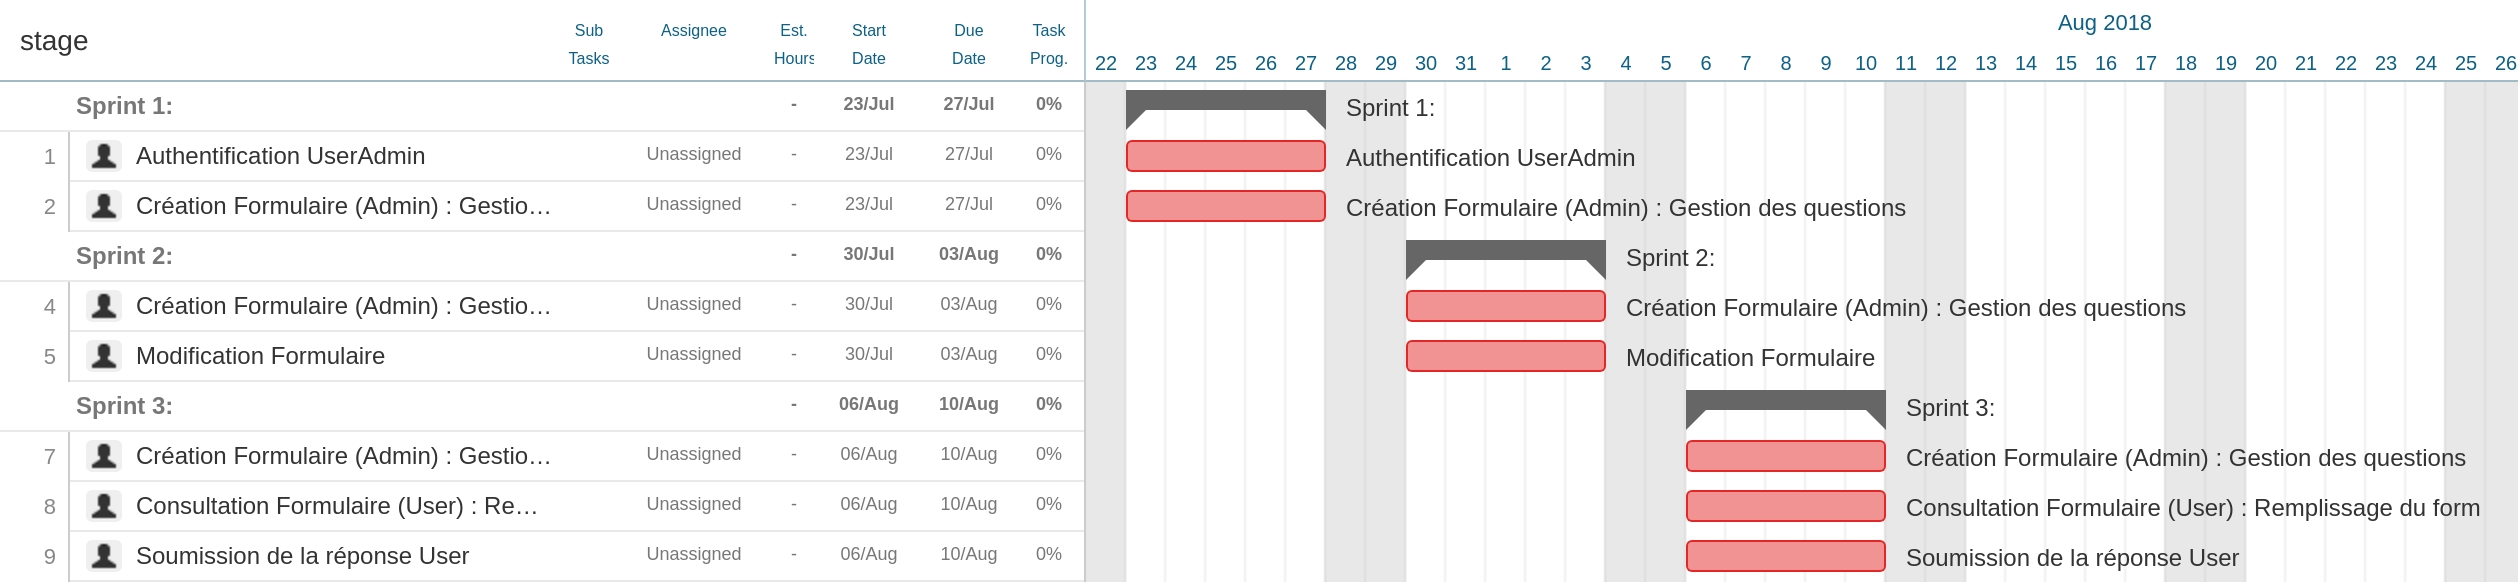
\includegraphics [width=18cm,height=9cm] {img/GANTTdiag.jpg}
            \caption{Diagramme de GANTT}
            \label{figger}
        \end{center}
    \end{figure}
    
\section{Conclusion}
Tout au long de ce chapitre, nous avons pu situer le cadre général de notre stage, à savoir la présentation du travail et ses objectifs, la société d’accueil et le cahier des charges proposé. Nous avons étayé aussi le choix du langage et la méthode de travail à utiliser.
Ce premier chapitre nous a introduit le contexte général du sujet à réaliser, le chapitre suivant sera entièrement consacré pour une étude conceptuelle du projet y compris l'analyse et l'étude des besoins du projet et son conception.
        \clearpage
        
        \chapter{Analyse et spécification des besoins}

\section{Introduction}
Nous réservons le deuxième chapitre pour détailler le cadre du projet, par une étude et critique de l’existant puis présenter la solution envisagée par le cahier de charges proposé.
Ensuite,nous allons identifier les acteurs qui interagissent directement avec l’ensemble de notre application, puis nous présentons dans ce qui suit les besoins fonctionnels classés par acteur ainsi que les besoins non fonctionnels et le diagramme de classes et séquence du projet.
% Une section
\section{\'Etude et critique de l'existant}
Il existe de nos jour un grand nombre de logiciels de génération de formulaires en ligne, ces  logiciels d’enquête  qui ne nécessitent aucune connaissance en programmation, peuvent s’avérer très utiles dans l’élaboration d’un questionnaire en ligne.\\
Ces derniers peuvent être des bons outils pour répondre mieux à nos attentes mais peuvent par conséquent présenter certaines limites dans leur utilisation.\\
Nous proposons une liste non exhaustive de quelques outils de génération de formulaires en ligne qui sont les leaders dans le marché accompagnée d'une brève analyse des avantages et des limites :\\
- \textbf{Google Forms}: Les formulaires Google sont des outils très pratiques par leur simplicité de mise en place et leur exploitation, aucune limite au nombre de questionnaires et au nombre de répondants, ils sont idéals pour les débutants, par conséquent la mise en page des questionnaires n’est que très peu personnalisable et ses serveurs sont localisés à l’étranger, les données seront soumises aux lois de ce même pays qu'il faut vérifier que cela soit compatible avec les exigences des comités d'éthiques.\\%te7ki b s3ib xD
- \textbf{LimeSurvey}: Un générateur de formulaire permet de créer rapidement et de manière intuitive de puissants questionnaires et enquêtes en ligne. Le questionnaire est hébergé sur le serveur de l’utilisateur mais ça reste toujours un outils considéré comme non personnalisé et que nous pouvons pas l'intégrer facilement dans des applications privées. 

\section{Solution proposée}
Tenant compte de l’étude approfondie de l’existant nous allons élaborer la solution proposée par SOFIA Technologies à mettre en oeuvre qui réponds à ces deux exigences : \\
- Développer un générateur de formulaire personnalisé qui garanti les besoins définis dans le cahier des charges.\\
- Proposer la solution sous forme d'un POC qui a pour but d’analyser sur une période définie et en situation réelle la mise en place d’une solution d’affichage dynamique dans le but de valider la conformité du projet avec les objectifs fixés, et plus globalement, avec le cahier des charges élaboré {Proof Of Concept \cite{webArticle2}}
\section{Identification des acteurs du système}
Les acteurs sont les entités externes qui interagissent avec le système. Notre projet comporte principalement deux acteurs :\\
- \textbf{Administrateur}: C’est l’acteur principal, il est responsable de la gestion des utilisateurs, des formulaires et des réponses de l’application.\\
- \textbf{Utilisateur}: Il s’agit d’un acteur principal aussi, il assure la consultation et la soumission des formulaires disponibles.
        
\section{Identification des besoins}
    % Une sous section
    \subsection{Besoins fonctionnels}
Les besoins fonctionnels représentent les services qui doivent être offerts et qui seront implémentés par l’application. Ainsi, cette application doit couvrir principalement les
besoins fonctionnels suivants :
\begin{itemize}
    \item S’authentifier : L’utilisateur peut créer un compte personnel et se connecter grâce à son login et mot de passe.
\end{itemize}
Pour l’administrateur :
\begin{itemize}
    \item Gérer les formulaires et leurs questions: cette étape consiste à faire les opérations CRUD pour un formulaire donné.
    \item Consulter la liste des formulaires : il peut visualiser tous les formulaires qu'il a crées.
    \item Consulter l’ensemble des réponses : L’administrateur peut consulter les réponses des utilisateurs aux différents formulaires qu'il a crées,les supprimer et même télécharger la liste des réponses.
\end{itemize}

Pour l'utilisateur:
\begin{itemize}
\item Consulter la liste des formulaires : L’utilisateur peut visualiser tous les formulaires crées par l’administrateur.
\item Soumettre un formulaire: il peut répondre aux questions d'un formulaire, modifier ses réponses et les soumettre.
\end{itemize}
    % Une deuxième sous section1
    \subsection{Besoins non fonctionnels}
      Dans le cadre de ce travail, notre application devra être :
\begin{itemize}
 \item  \textbf{Performante} : l’administrateur ne peut gérer les formulaires et les utilisateurs qu’après authentification et même cas pour les utilisateurs pour répondre aux formulaires.
 \item \textbf{Ergonomique } : Il s’agit d’une application présentant des interfaces utilisateur conviviales bien structurée et simple à manipuler
 \item  \textbf{Rapide et fluide} : Ce besoin envisage avec une vitesse de navigation minime, temps de réponse rapide et temps d’affichage optimisé.
\end{itemize}
\section{Conception}
\subsection{Le diagramme de classe et diagramme de cas d’utilisation}
Dans cette section nous présentons le diagramme de cas d’utilisation des fonctionnalités déjà mentionnées ainsi que le diagramme de classes.\\
Le diagramme de cas d’utilisation général de la figure  (\ref{casgeneral}) permet d’avoir une vue globale du fonctionnement de notre système à réaliser.
\begin{figure}[H]
    \centering
    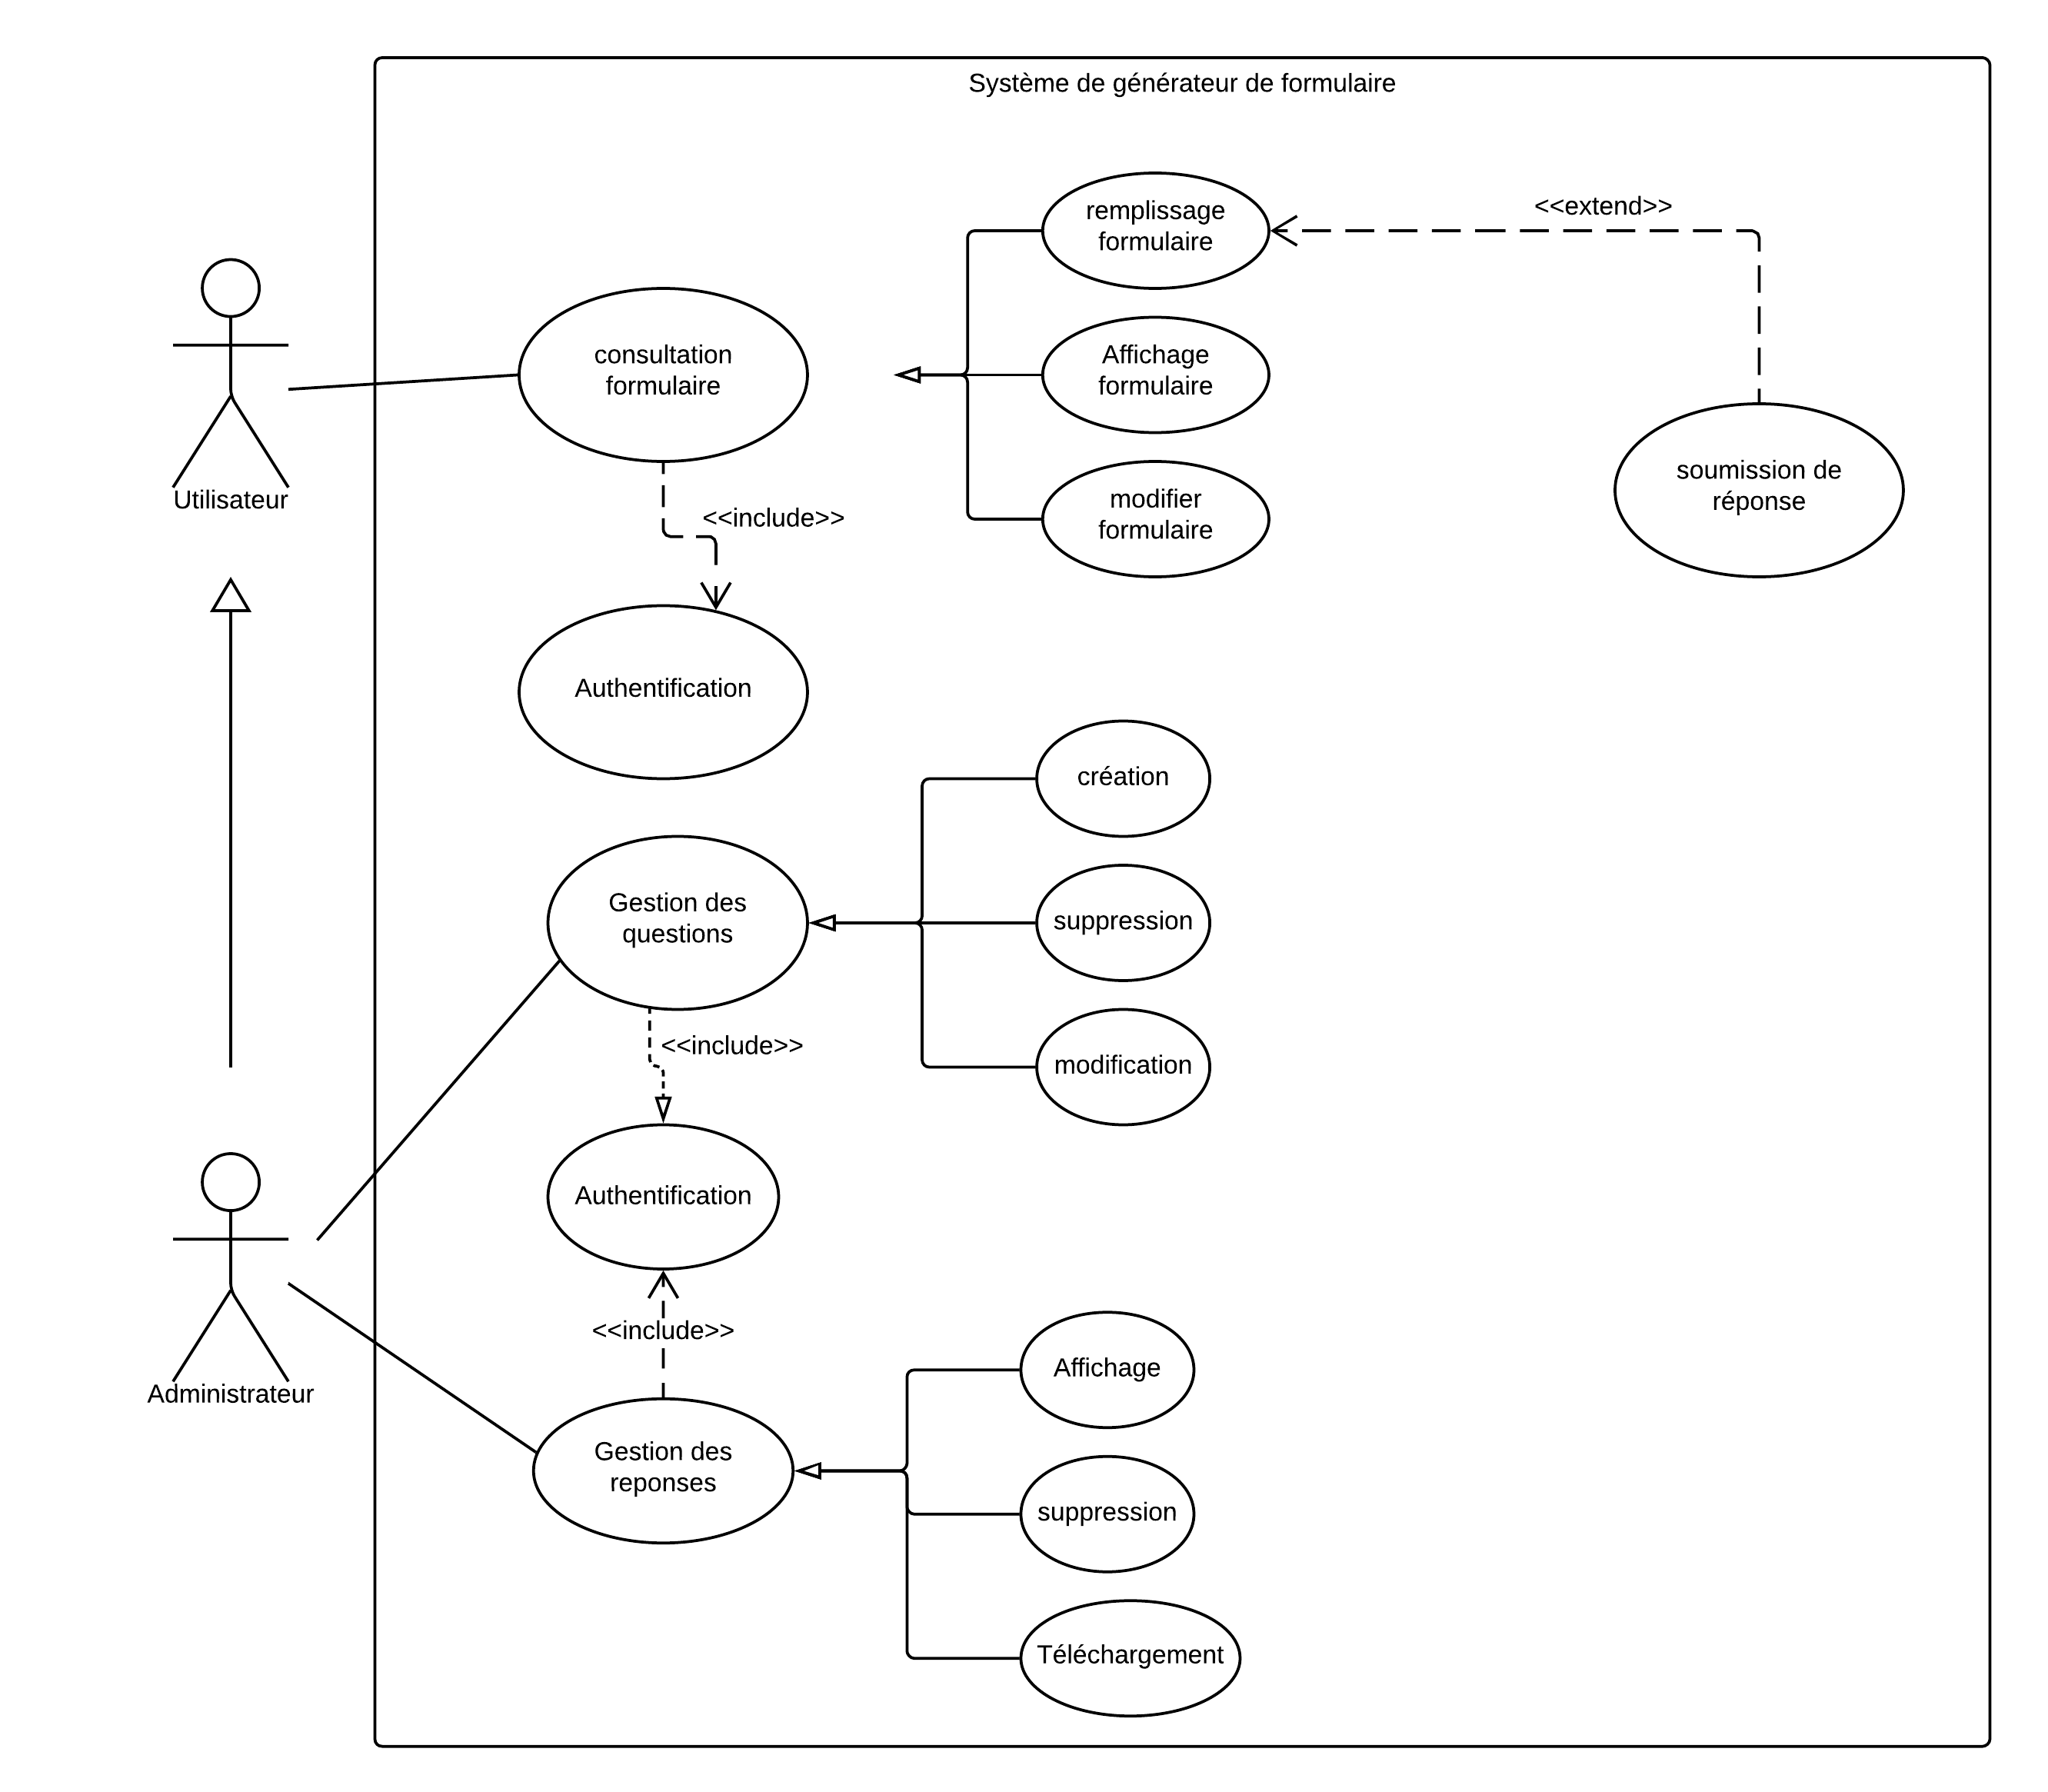
\includegraphics[width=14cm, height=8cm]{img/Diag_usecase.png}
    \caption{Digramme de cas d'utilisation général}
    \label{casgeneral}
\end{figure}

La figure (\ref{ClasseGeneral}) présente le diagramme de classes de notre projet.
\begin{figure}[H]
    \centering
    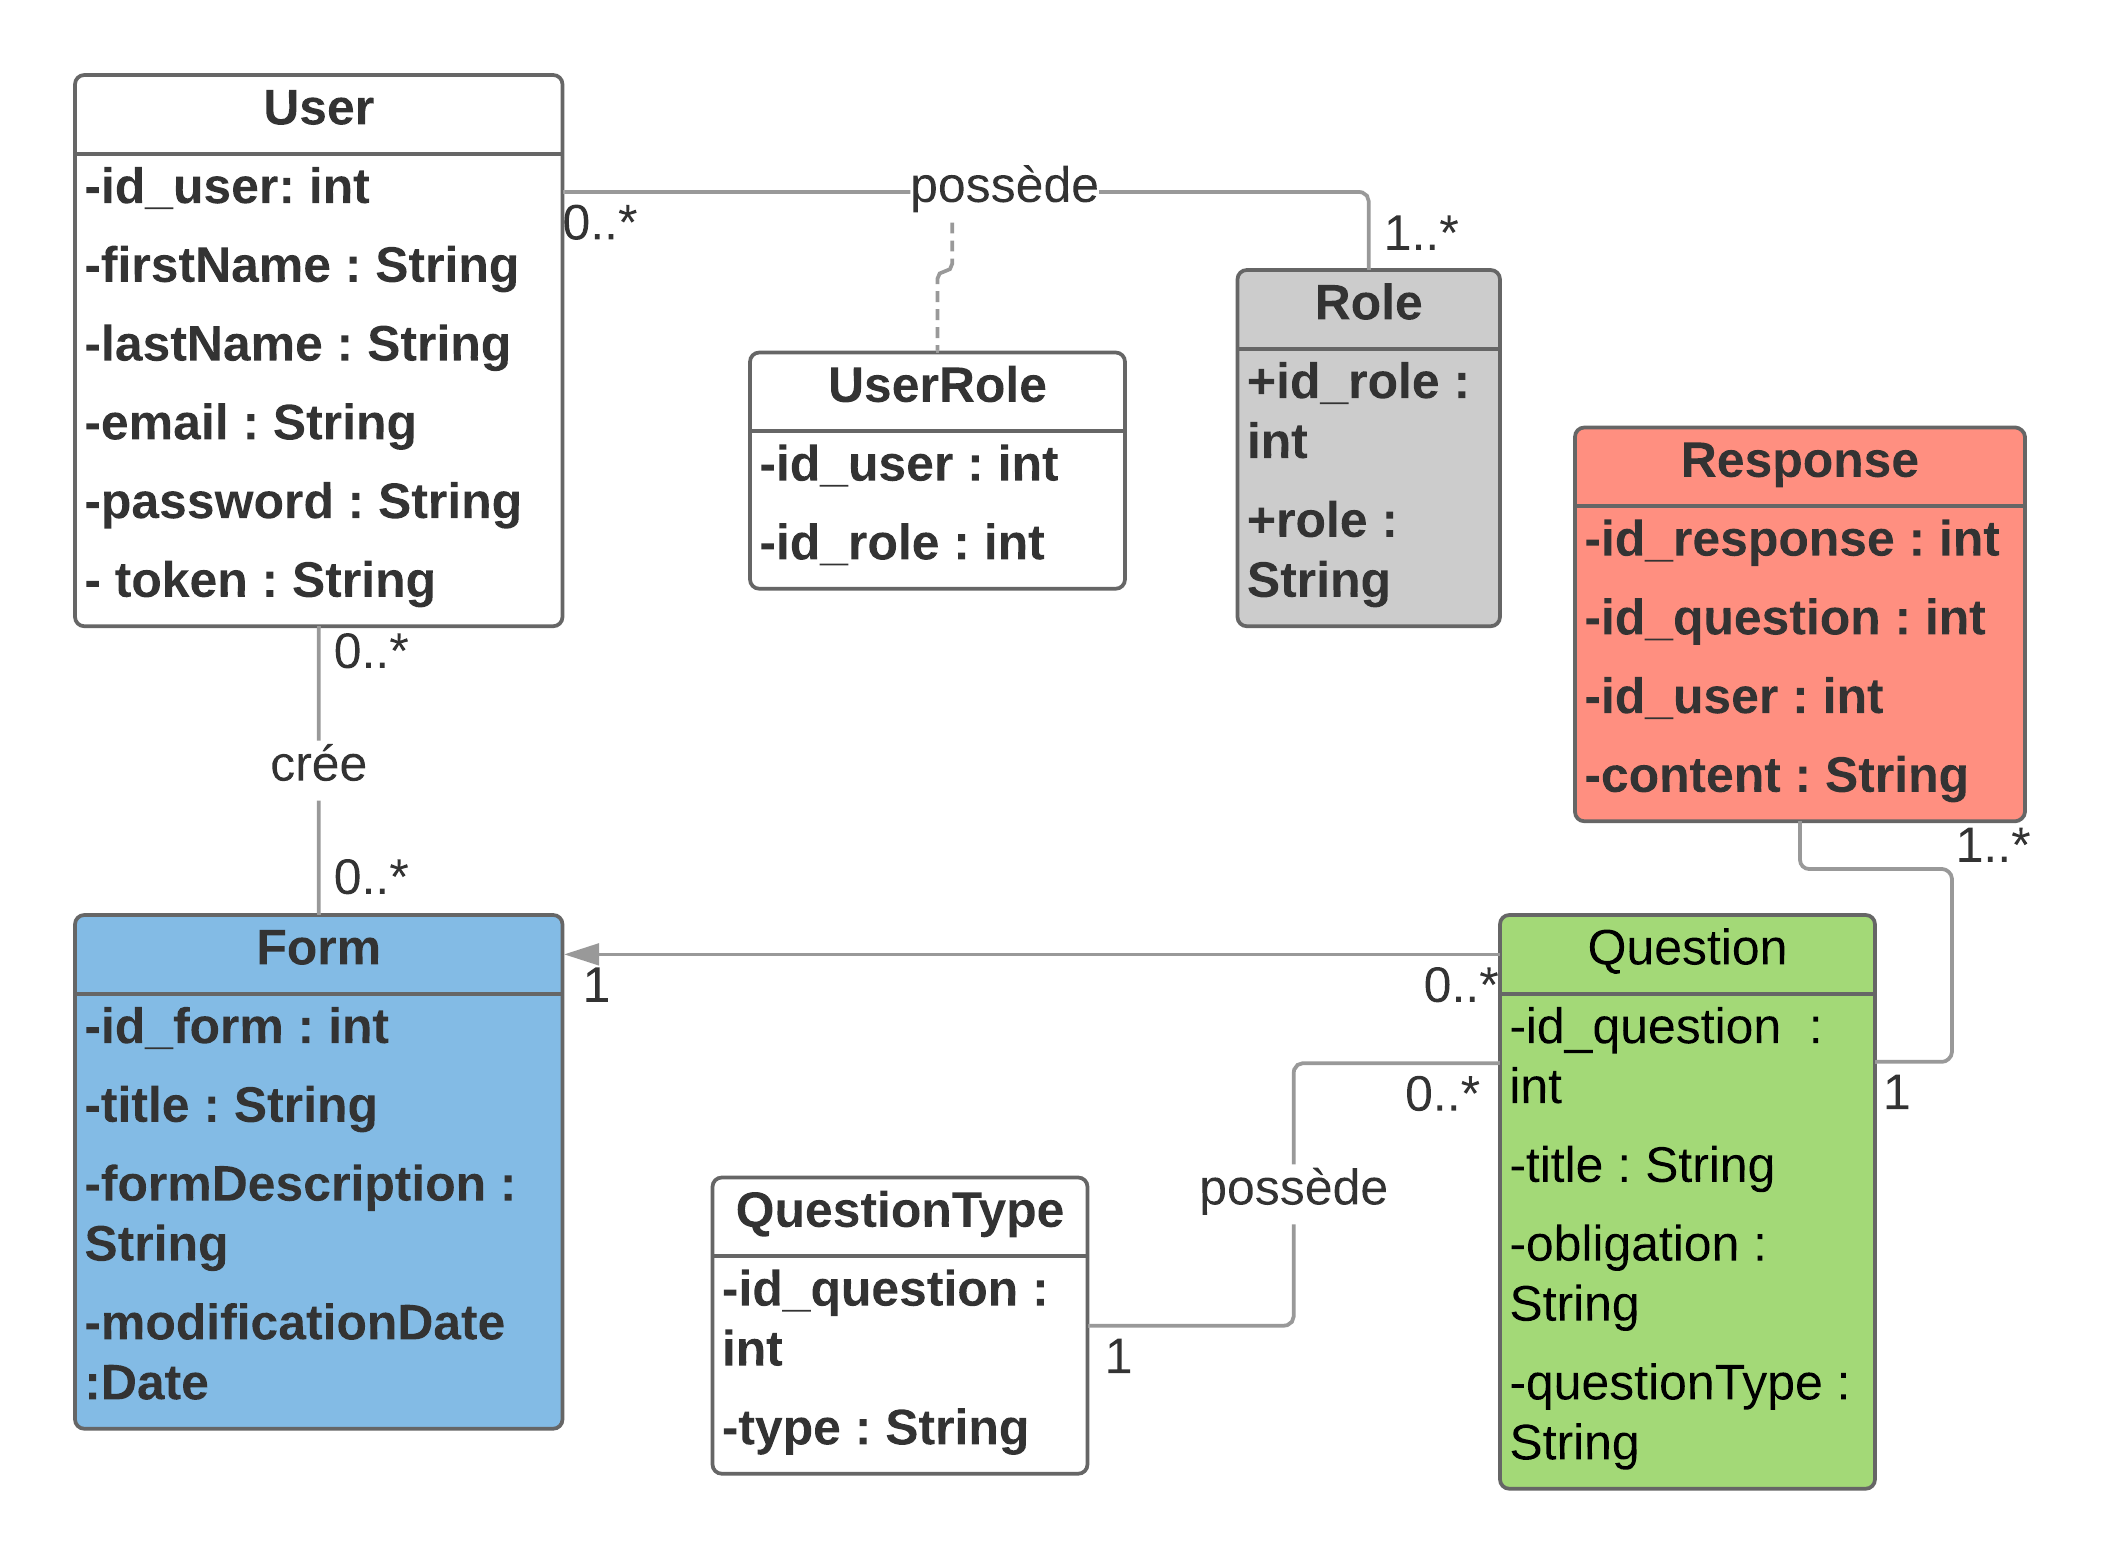
\includegraphics[width=14cm, height=8cm]{img/DiagClasse.png}
    \caption{Digramme de classes général}
   \label{ClasseGeneral}
\end{figure}

\subsection{Identification des scénarios}
  
Le tableau \ref{tabGererOffre} présente la description détaillée du cas d'utilisation "s'inscrire".
    \begin{longtable}{|p{4cm}|p{10.25cm}|}
	\hline
	\textbf{Nom} & Authentification\\ \hline
	\textbf{Acteur}& L'utilisateur. \\ \hline
	\textbf{Description} & Permettre aux utilisateurs de créer des comptes. \\ \hline
	\textbf{Pré-condition} & 1. L'utilisateur devrait consulter la page d'inscription.L'utilisateur ne doit pas être déjà enregistré.\\
	\hline \textbf{Scénario nominal} & 1. L'utilisateur saisit son username.\\
	& 2. L'utilisateur saisit son mot de passe.
	\\ \hline
	\textbf{Scénario d'exception} &  Si l'utilisateur saisit un email ou un username erroné, il sera invité à saisir son login de nouveau.\\ \hline
	\textbf{Post-condition} & L'utilisateur devient authentifié par l'intermédiaire d'un token.\\\hline
	\caption{ Description du processus d'inscription}\label{tabGererOffre}
	\end{longtable}
\section{Schéma de la base de données}
Pour pouvoir commencer la partie développement, il faut bien comprendre la structure de notre base de données c’est-à-dire les entités et les associations.\\
A l'aide du système de gestion de bases de données relationnelles MySQL, nous avons pu installer notre serveur de base de données. La figure \ref{schémaDB} illustre le schéma de la base de données en détaillant les attributs de chaque table.
 \begin{figure} [H]
    \centering
         \begin{center}
             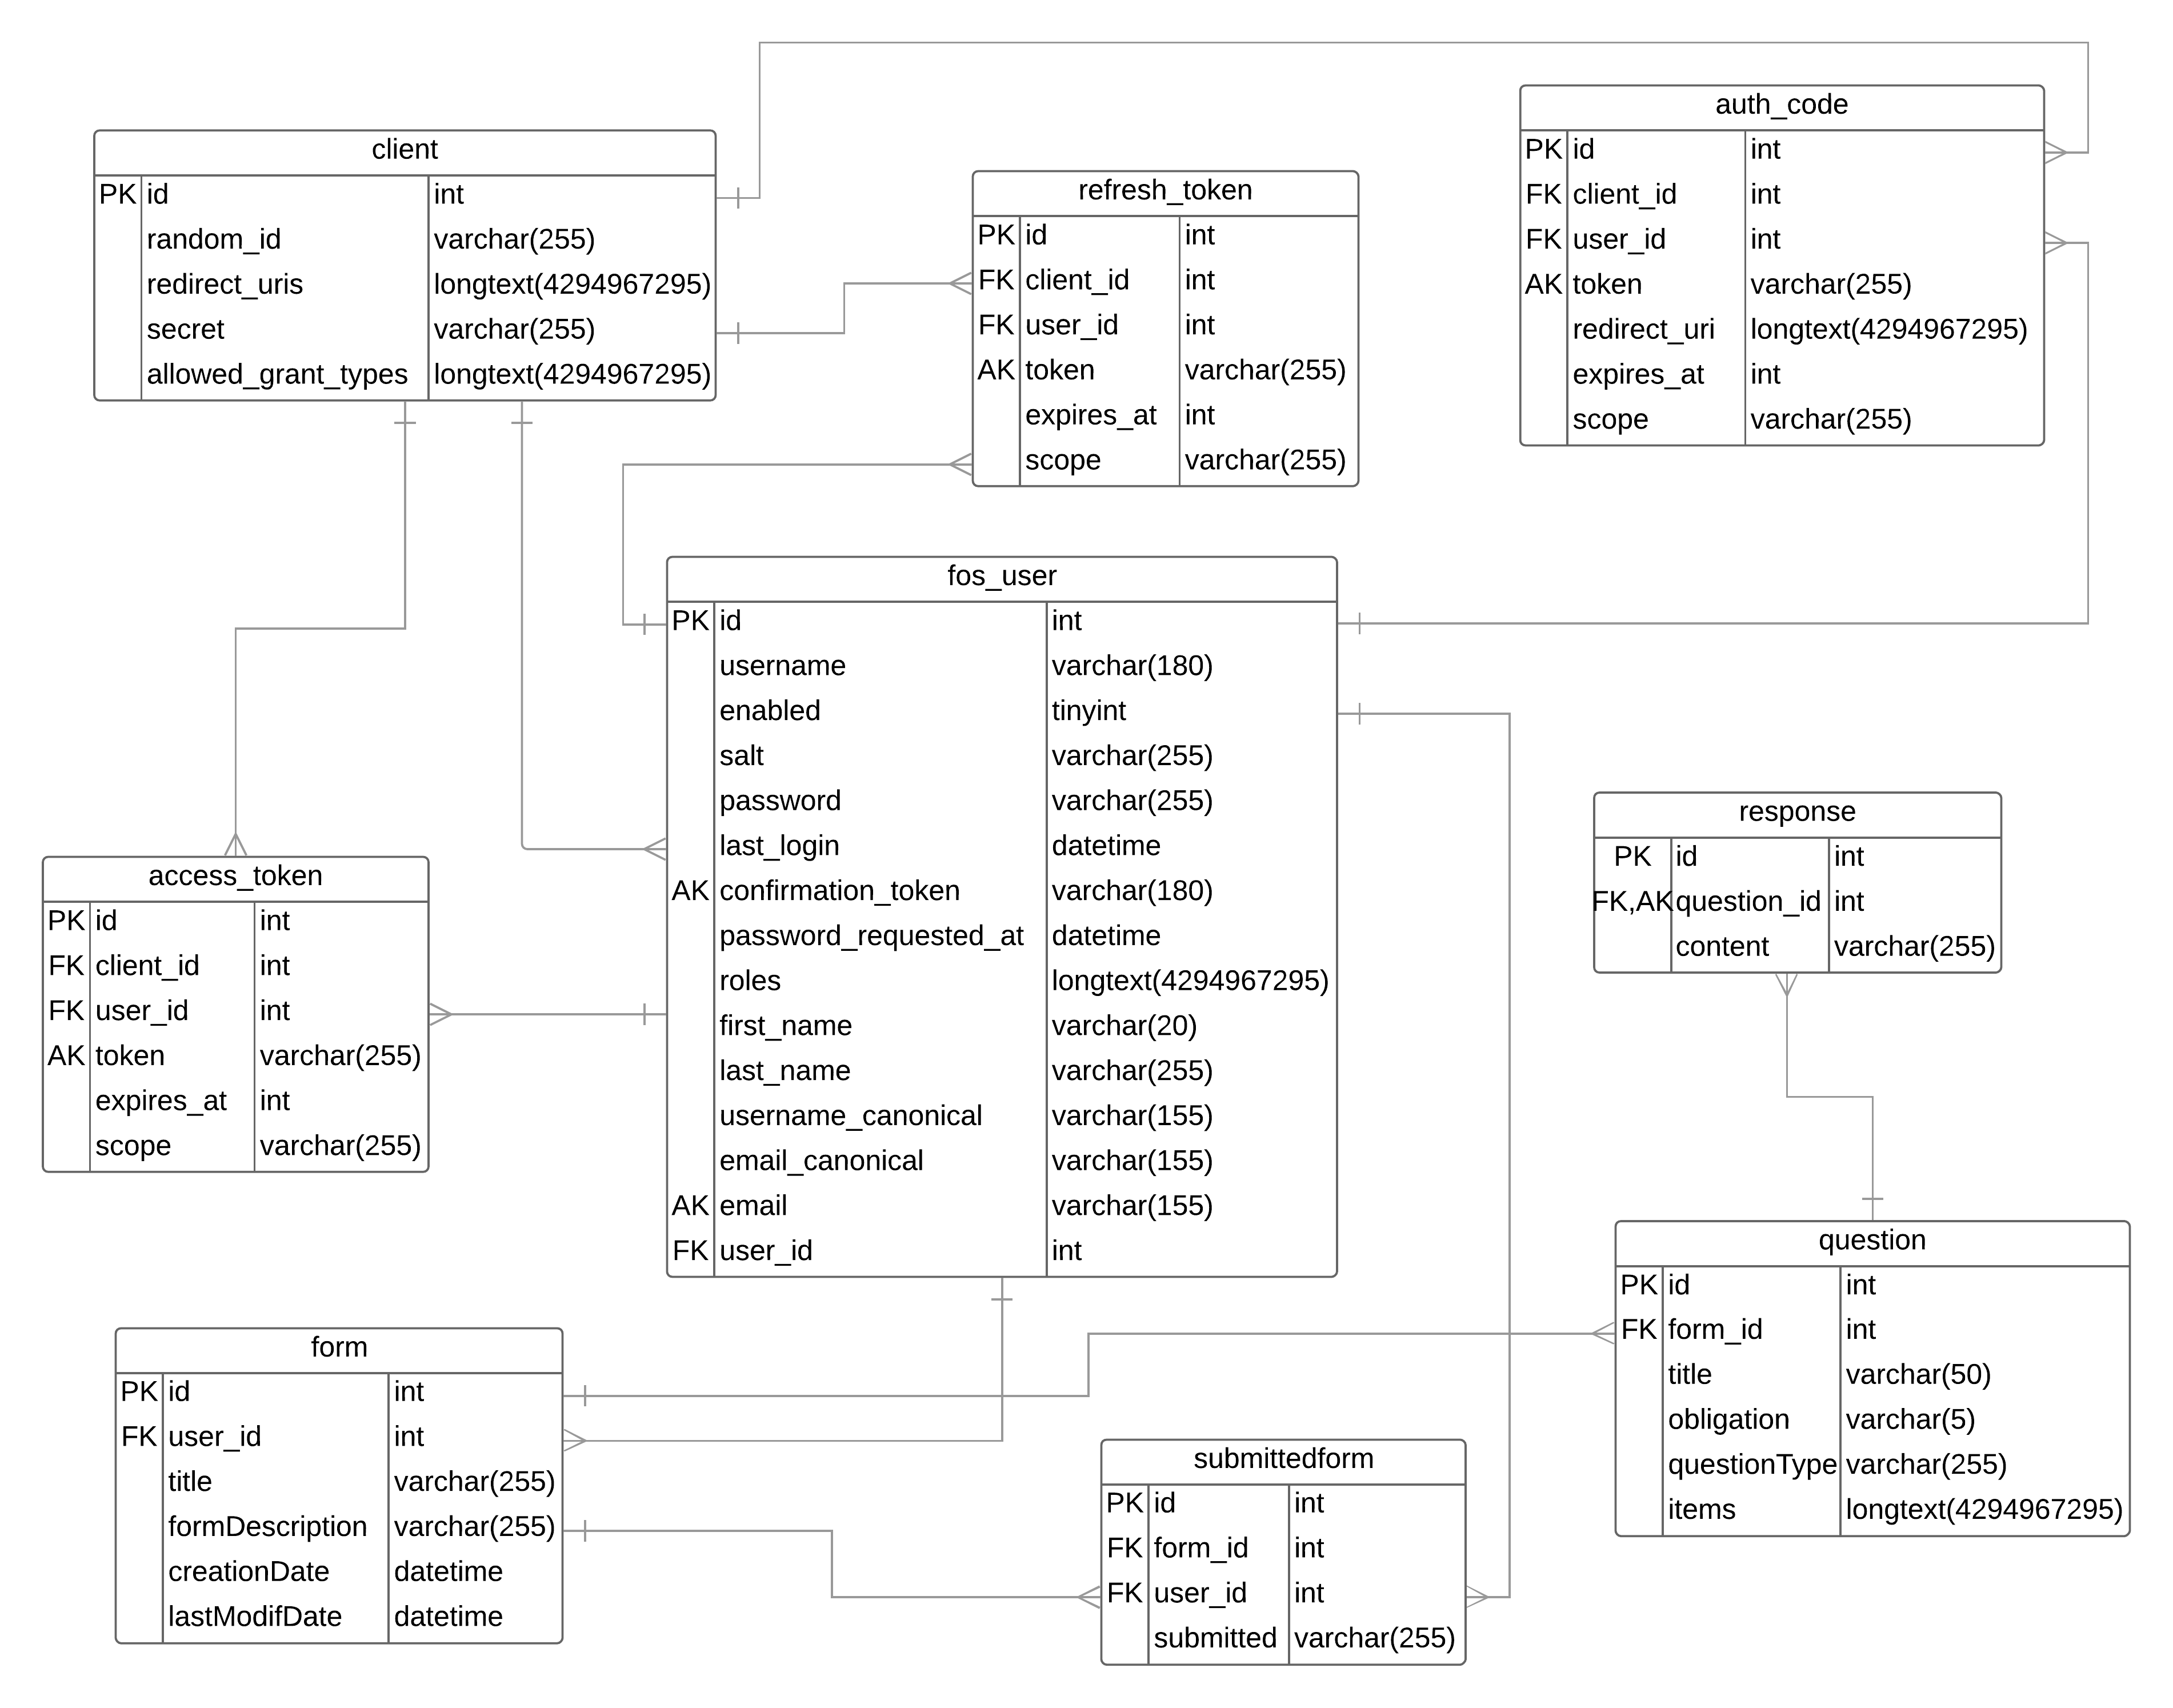
\includegraphics [width=16cm,height=9cm] {SprintImage/DB_schema}
            \caption{Schéma de la base de données}
            \label{schémaDB}
        \end{center}
    \end{figure}
\subsection{Diagrammes de séquence}
Dans cette partie, nous allons modéliser les fonctionnalités du premier sprint sous forme d’une séquence de messages échangés entre l’acteur et le système.\\
\textbf{Diagramme de séquence système « S’authentifier »}\\
La figure \ref{séqAuth} représente l’enchaînement du cas d’utilisation « S’authentifier ». Le user ou l'administrateur demande son authentification en saisissant ses identifiants
(username, password). Le système vérifie si les identifiants sont corrects ou non. Une fois les coordonnées sont valides,un token(jeton d'authentification) est envoyé du back-end et le User sera amené à la page d’accueil. Dans le cas contraire, un message d’erreur sera affiché en lui indiquant le problème.
\begin{figure} [H]
    \centering
         \begin{center}
             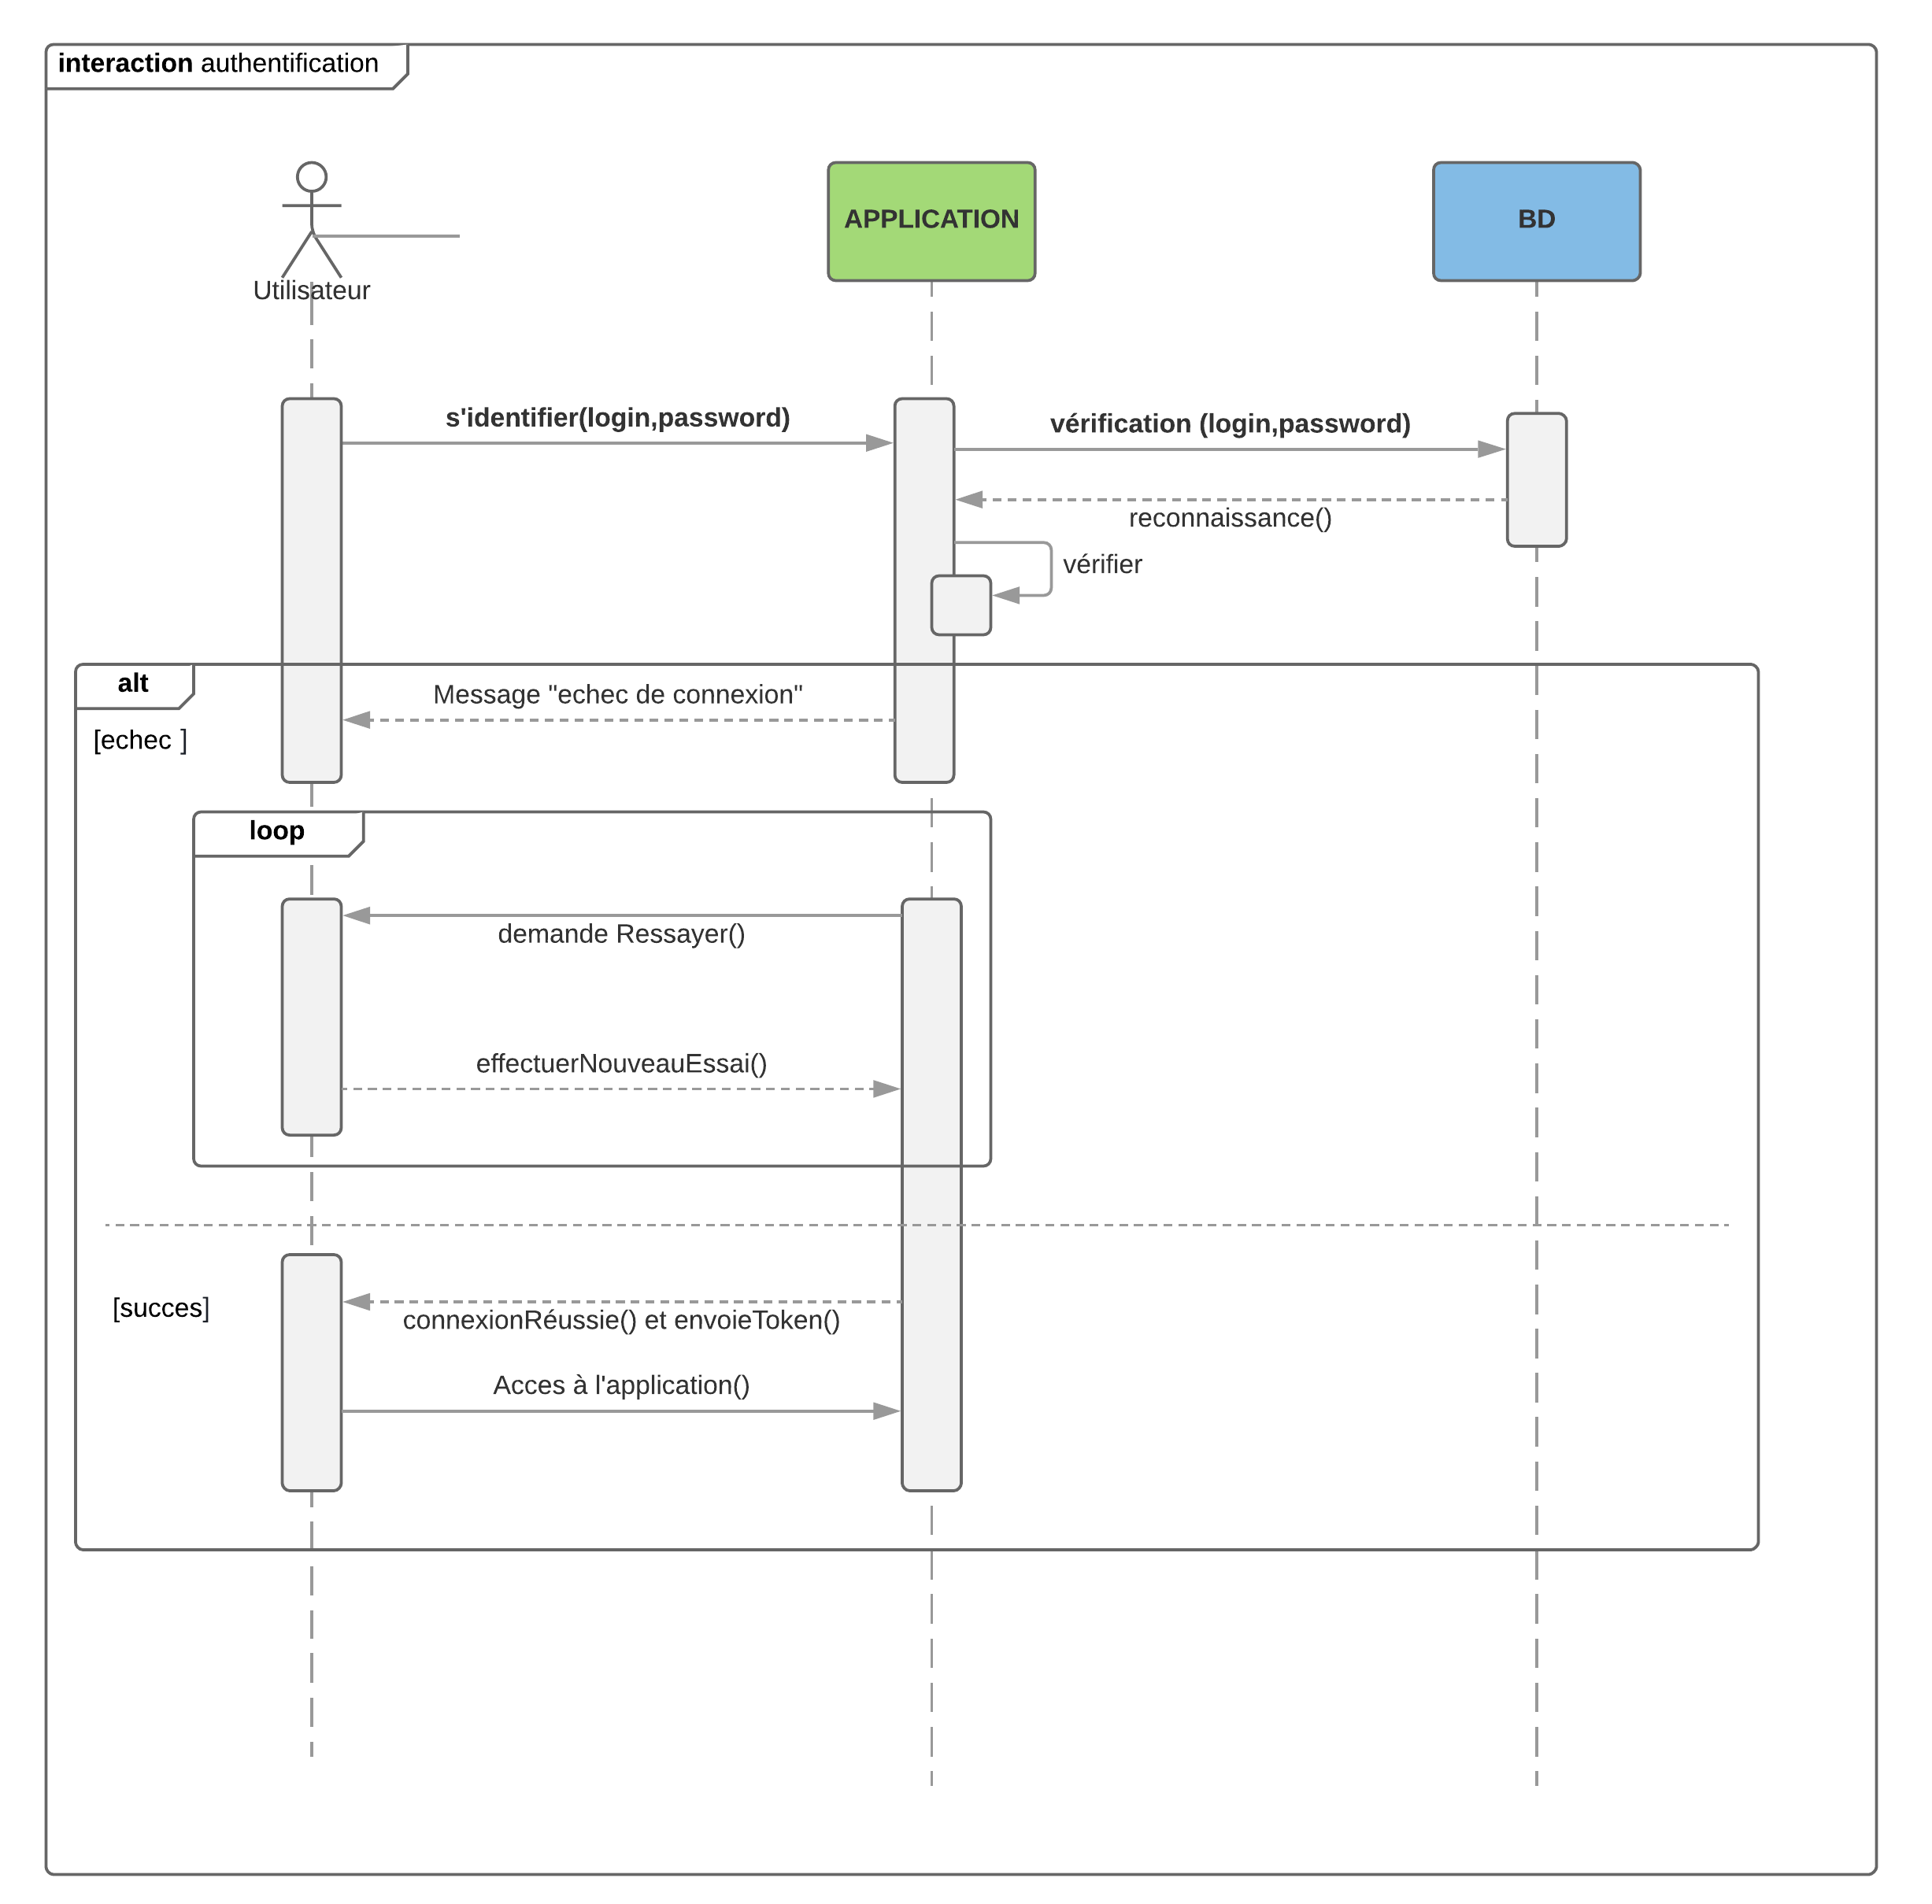
\includegraphics [width=15cm,height=11cm] {SprintImage/Diagramme_seq_Auth}
            \caption{Diagramme de séquence système « S’authentifier »}
            \label{séqAuth}
        \end{center}
    \end{figure}
    \newpage
\subsection{Diagramme de séquence système « Soumettre la réponse d'un formulaire »}
Le diagramme de la figure \ref{fig4}, représente les étapes qu'un utilisateur doit suivre afin de soumettre sa réponse à un questionnaire choisit.  
  \begin{figure} [H]
    \centering
         \begin{center}
             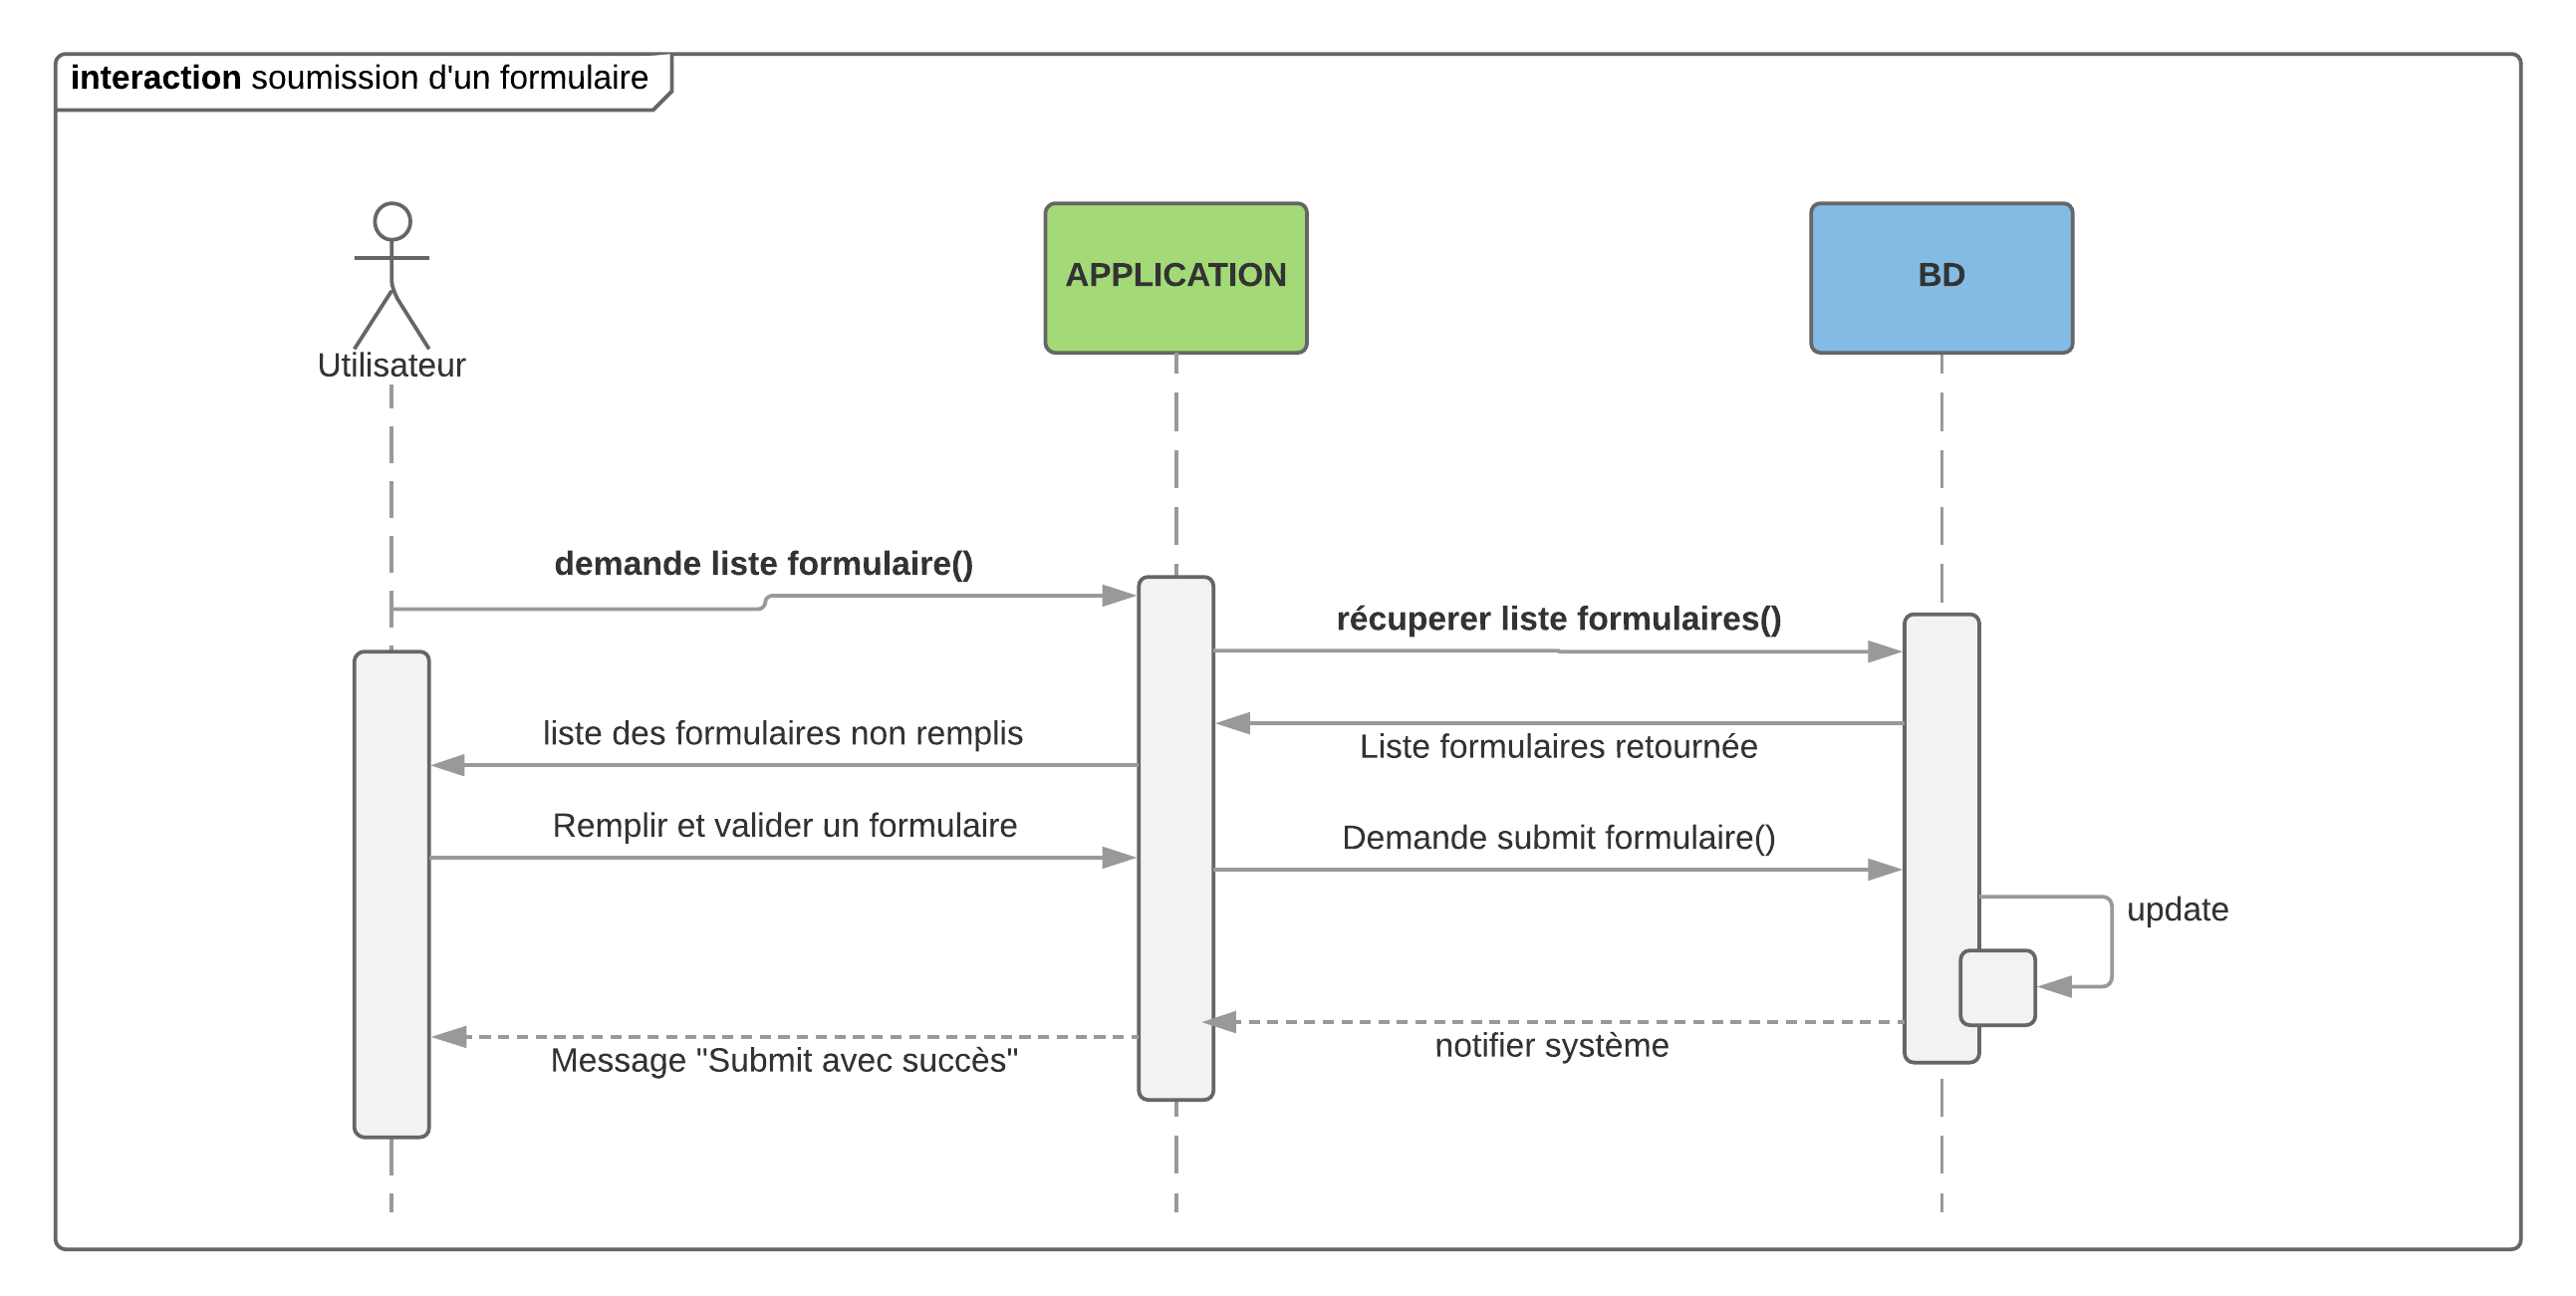
\includegraphics [width=16cm,height=7cm] {SprintImage/Diagramme_seq_formSubmit.png}
            \caption{Soumission de la réponse par le User }
            \label{fig4}
        \end{center}
    \end{figure}
\newpage
\subsection{Diagrammes de séquence système « Création formulaire »}
La figure \ref{form2} représente l’enchaînement du cas d’utilisation « Création Formulaire ».
\begin{figure} [H]
    \centering
         \begin{center}
             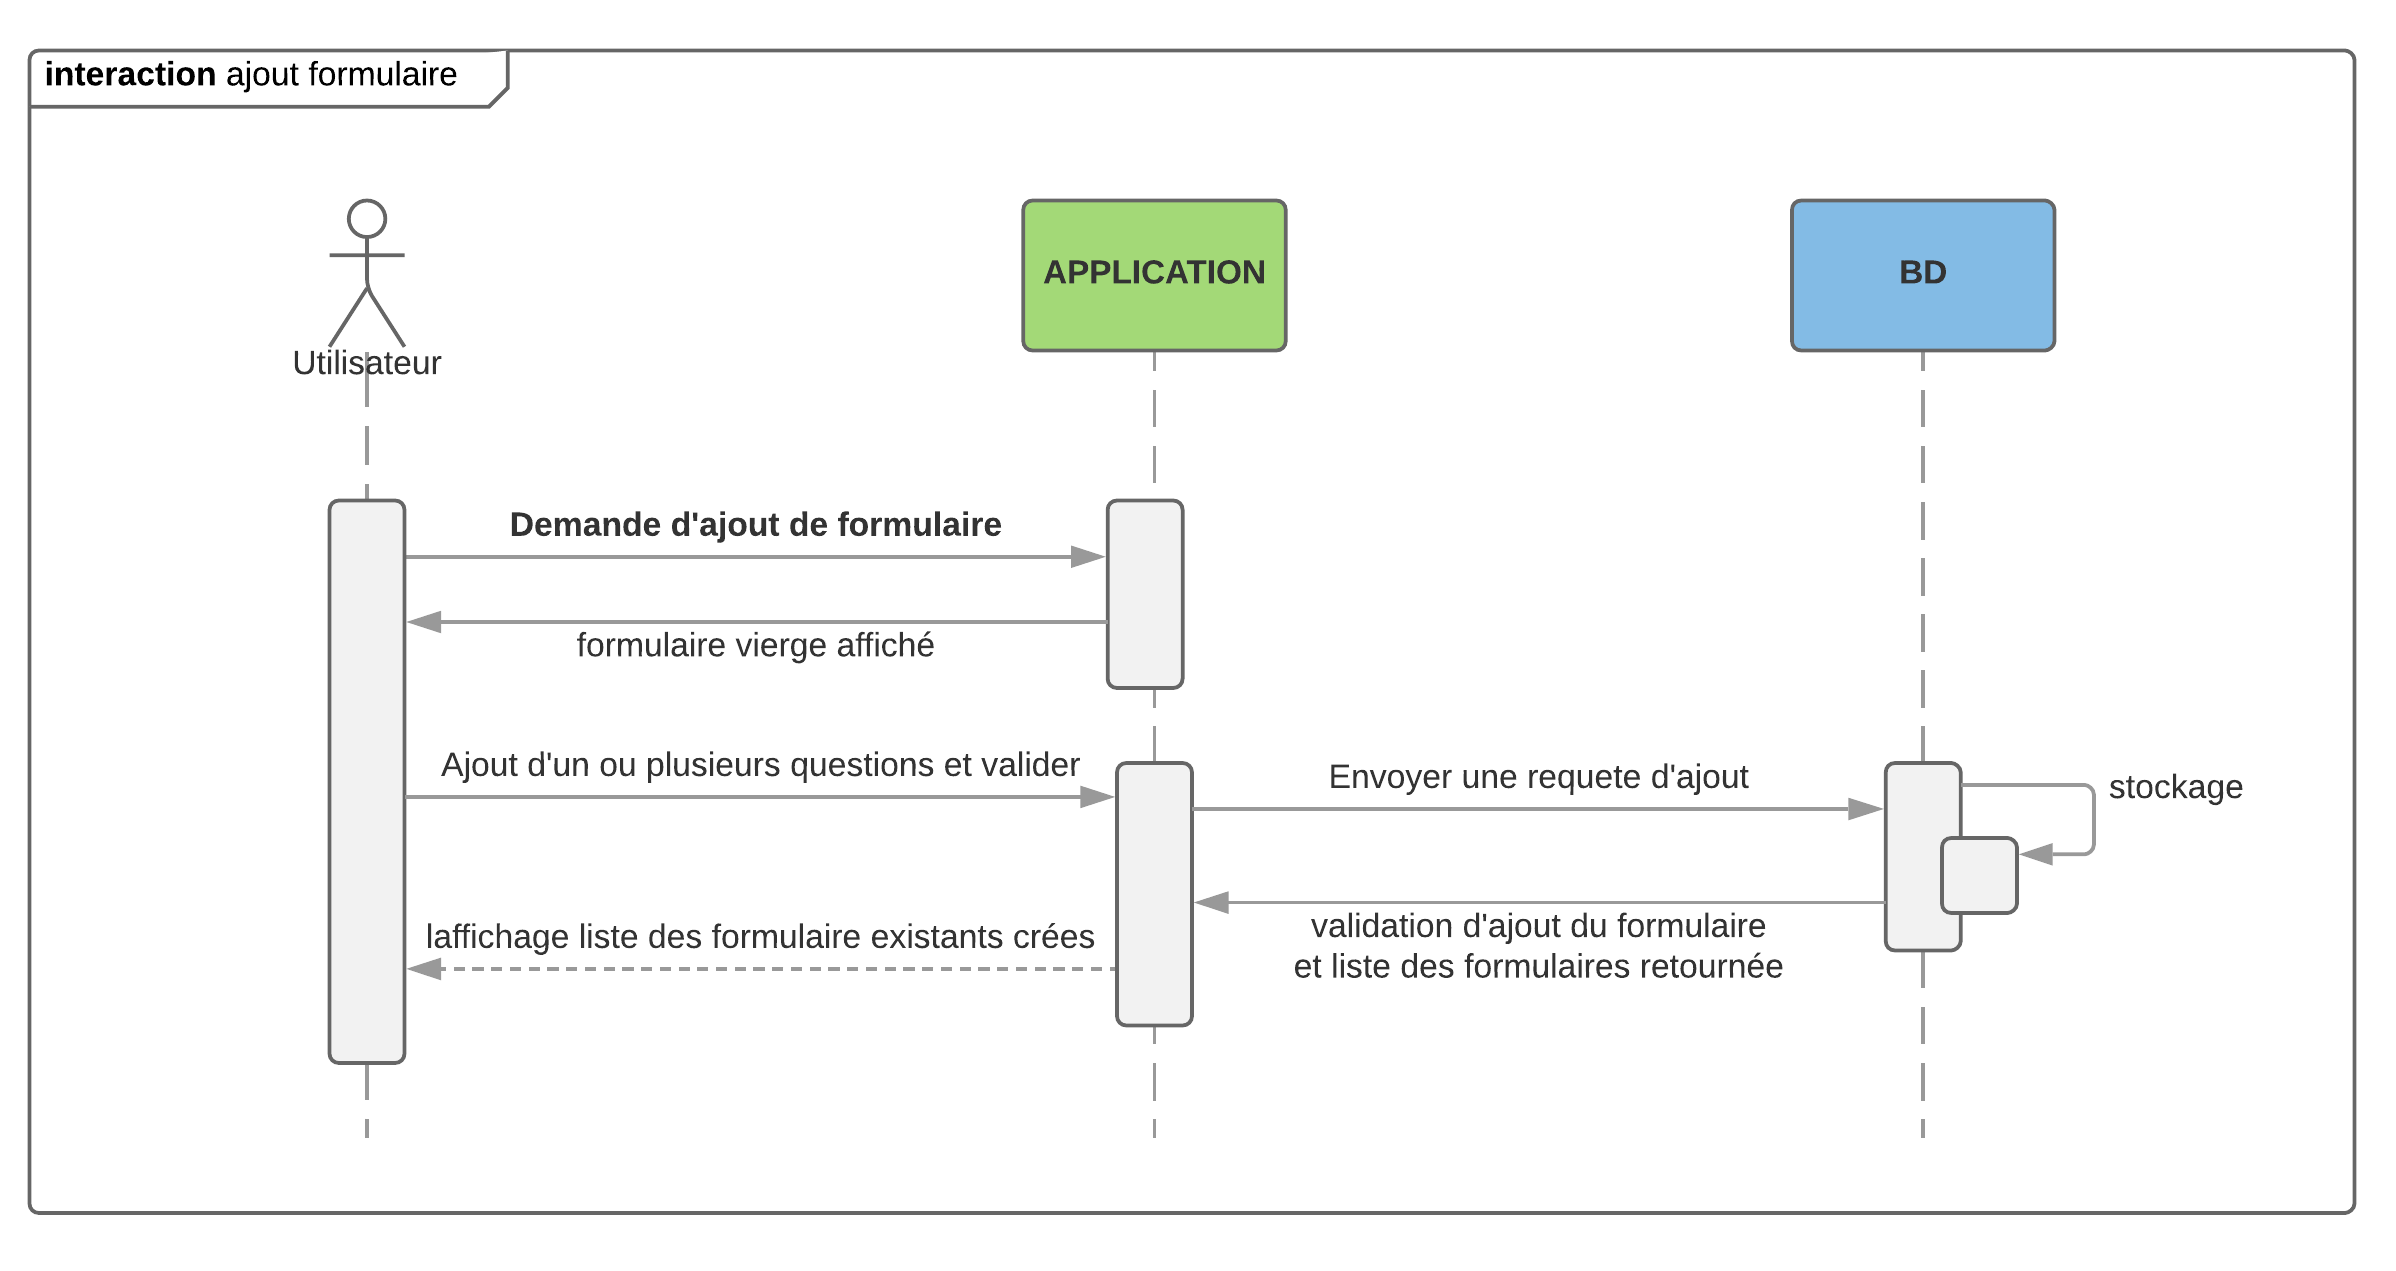
\includegraphics [width=16cm,height=9cm] {SprintImage/Diagramme_seq_ajoutForm.png}
            \caption{Mur de la création d'un formulaire}
            \label{form2}
        \end{center}
    \end{figure}
\section{Conclusion}
    Dans ce chapitre, nous avons précisé les besoins fonctionnels et non fonctionnels de l’application pour bien comprendre les différentes caractéristiques de notre système, ainsi que leur conception.
\newline
Dans le prochain chapitre, nous allons passé à la partie de réalisation des différents sprints tout en détaillant le choix des technologies utilisées.
        \clearpage
        
        \chapter{Réalisation}
	
\section{Introduction}
Ce chapitre constitue le dernier volet de ce rapport, il traite la phase qui a pour objectif l’implantation de notre application. Nous commençons par la description de l’environnement logiciel utilisé pour développer notre solution et les différentes fonctionnalités réalisées. Ensuite nous terminons par exposer l'écart entre la réalisation réelle et les taches planifiées au niveau du premier chapitre.
\section{Environnement de développement}
Afin de construire notre application, nous avons utilisé un ensemble de Framework, environnement de développement et outils
de conception, c'est ce que nous présenterons dans cette section.\\
L’environnement logiciel employé est le suivant :
\begin{itemize}
\item \textbf{WAMP}: Nous avons déployé nos intergiciels sous WAMP, vu qu’il propose les dernières mises à jour du langage PHP. En plus, il intègre plusieurs bibliothèques open source.
\item \textbf{Postman} : Nous avons testé nos services web grâce à l’outil Postman qui nous a permis de tester les requêtes HTTP et les interpréter en dehors du contexte métier.
\item \textbf{PHPStorm}: PhpStorm est un éditeur pour PHP, HTML, CSS et JavaScript, produit par JetBrains.
Il est compatible avec Git ce qui a facilité la procédure de gestion de versions au cours du développement de notre application.
Il est payant, sauf dans certains cas comme pour les étudiants ou les projets open source.
\end{itemize}

\section{Choix technologiques et langages utilisés}
Dans cette section, nous allons citer nos choix technologiques et les langages que nous avons utilisés pour mener à bien ce projet.
\subsection{WEB API RESTful}
Afin d’assurer l’interaction entre le back-end et le front-end de l'application, nous avons implémenté des services web PHP de type REST.
Les réponses sont sous format JSON puisque il est plus légère et facile à manipuler.
\subsection{Symfony 3.4}
Symfony est un framework MVC libre écrit en PHP 5. Il fournit des fonctionnalités qui permettent de faciliter et d’accélérer le développement d'un site web. 
\section{Planning réel du projet}
Nous présentons au cours de cette section, les durées réelles des tâches que nous avons
planifiées au niveau du premier chapitre.
Dû aux problèmes imprévus qui ont apparût lors de la réalisation de notre projet, nous
n’avons pas estimer les durées exactes de nos tâches.  \ref{fig6}.
\begin{figure} [H]
    \centering
         \begin{center}
             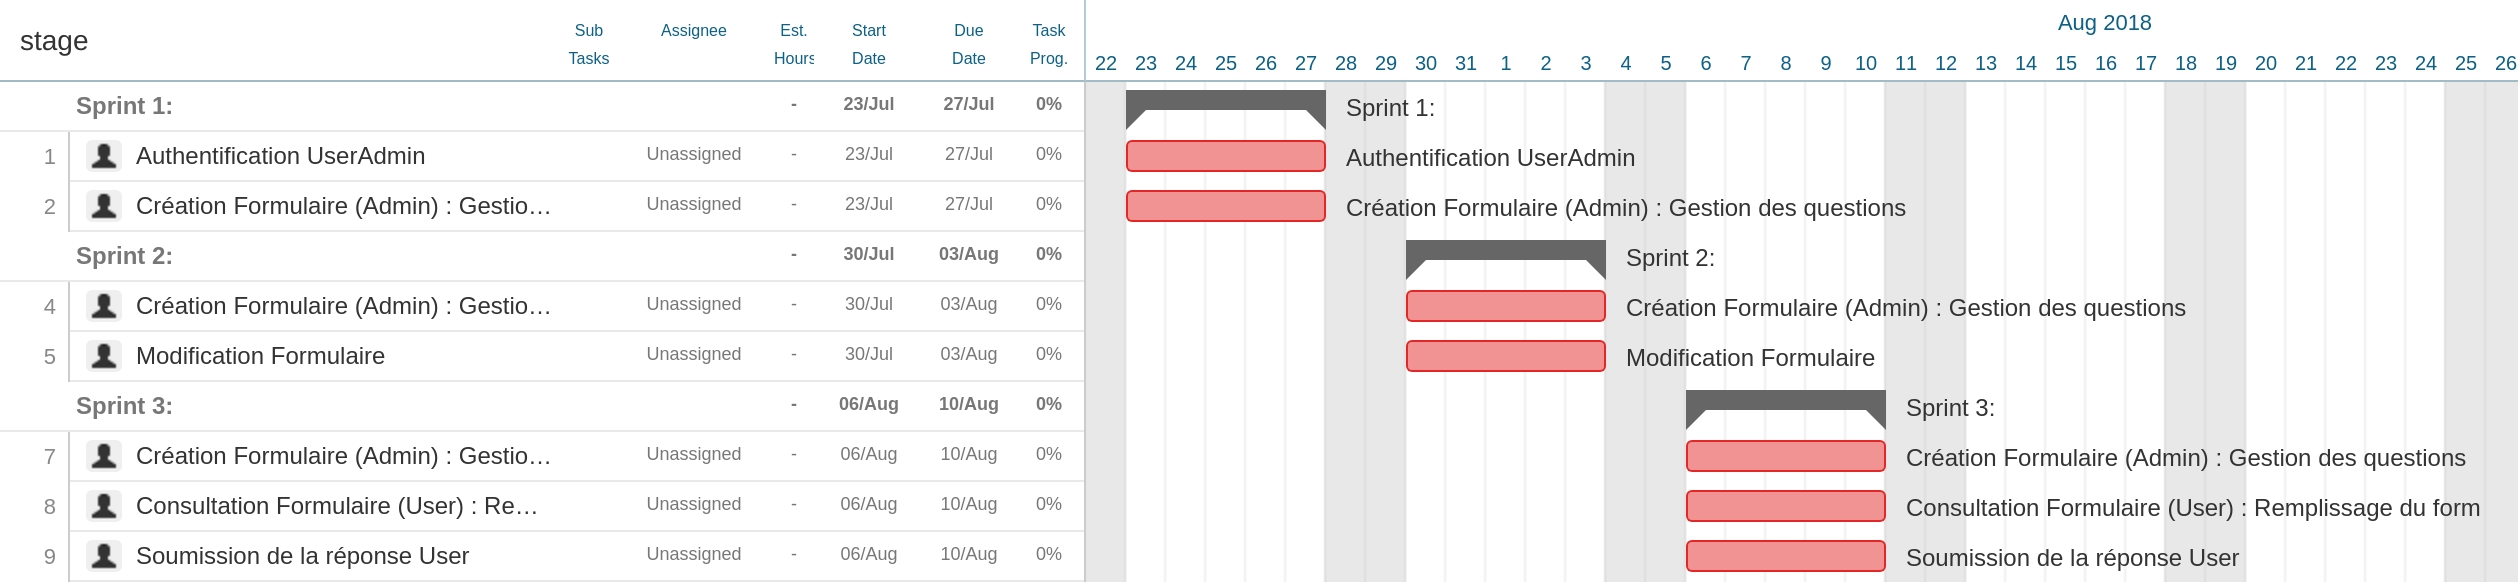
\includegraphics [width=16cm,height=8cm] {img/GANTTdiag.jpg}
            \caption{Réalisation en temps réel }
            \label{fig6}
        \end{center}
    \end{figure}
    
\section{Test des services web}
Les tests sont effectués grâce à l'outil Postman tout en introduisant l'url correspondant à l'API créee et la méthode HTTP utilisée avec un format de retour des données JSON.\\
La figure \ref{login} présente un succès d'authentification d'un administrateur.
\begin{figure} [H]
    \centering
         \begin{center}
             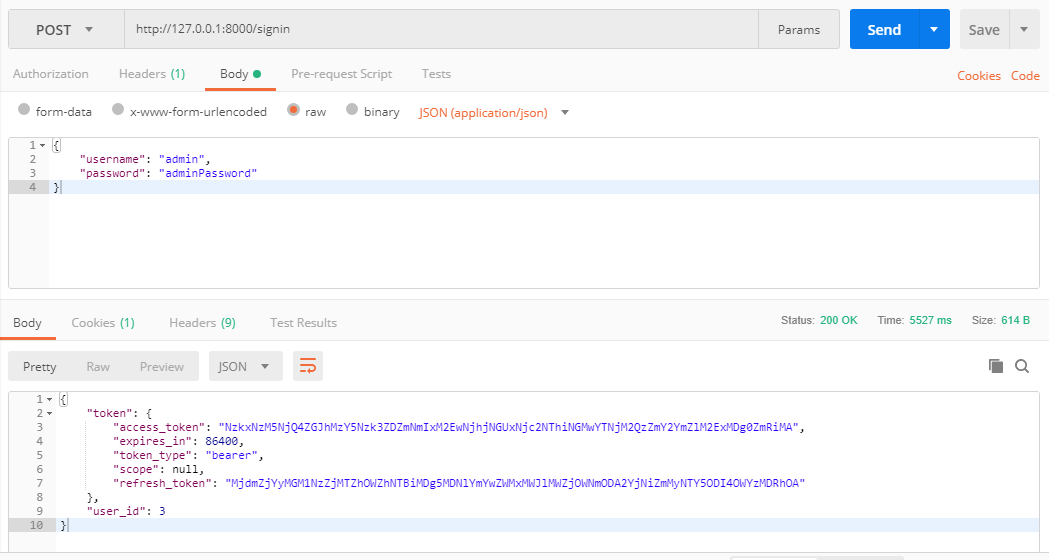
\includegraphics [width=16cm,height=9cm] {SprintImage/loginSuccess.PNG}
            \caption{Web Service "Signin"}
            \label{login}
        \end{center}
    \end{figure}
    
    La figure \ref{SerWeb1} illustre le service web permettant la soumission d'un formulaire, la figure \ref{SerWeb2} son affichage et la modification avec la figure \ref{SerWeb3}.

    \begin{figure} [H]
    \centering
         \begin{center}
             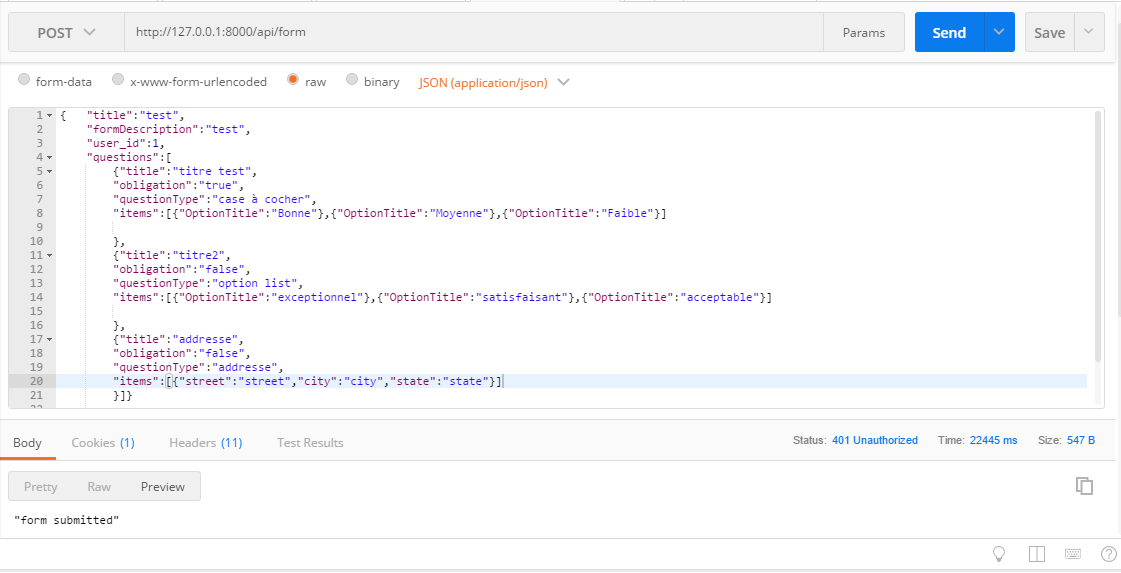
\includegraphics [width=16cm,height=9cm] {SprintImage/FormSubmitted.png}
            \caption{Web Service " Soumettre un formulaire"}
            \label{SerWeb1}
        \end{center}
    \end{figure}
    
    \begin{figure} [H]
    \centering
         \begin{center}
             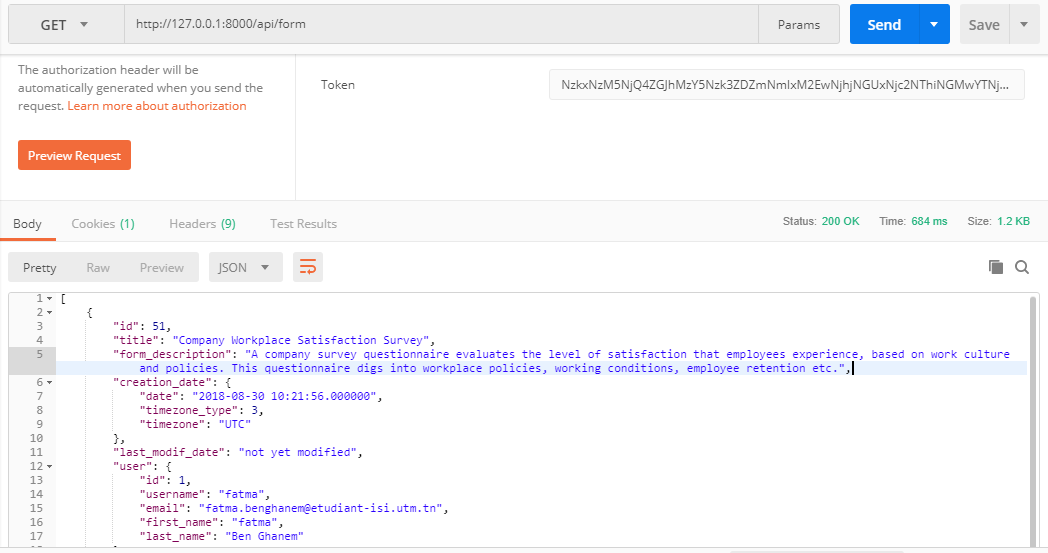
\includegraphics [width=16cm,height=9cm] {SprintImage/GetForms.PNG}
            \caption{Web service "affichage des formulaires"}
            \label{SerWeb2}
        \end{center}
    \end{figure}
    
    \begin{figure} [H]
    \centering
         \begin{center}
             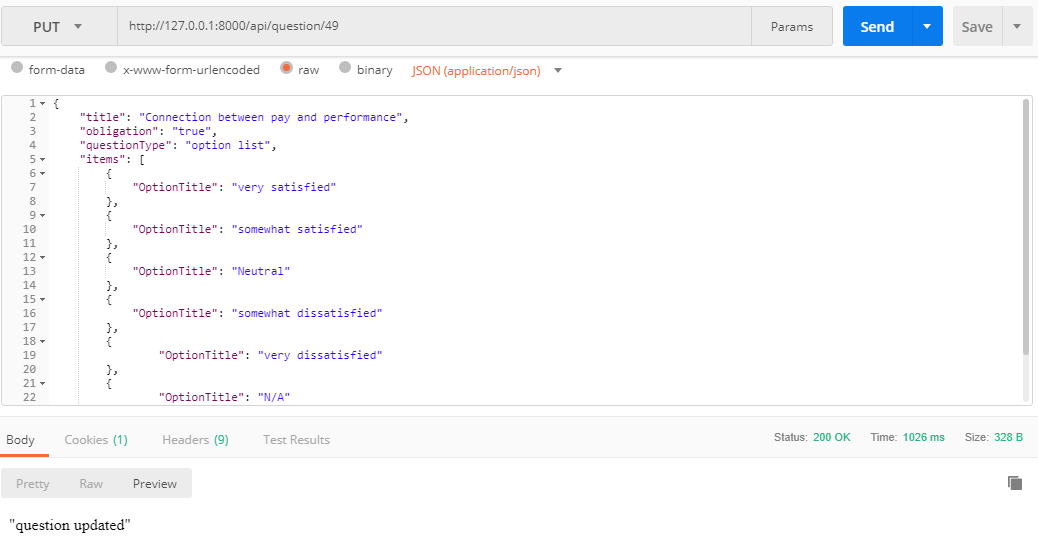
\includegraphics [width=16cm,height=9cm] {SprintImage/PutQuestion.PNG}
            \caption{Web service "modification formulaire"}
            \label{SerWeb3}
        \end{center}
    \end{figure}
    \newpage
     La figure \ref{fig5} illustre la soumission d'une réponse.
\begin{figure} [H]
    \centering
         \begin{center}
             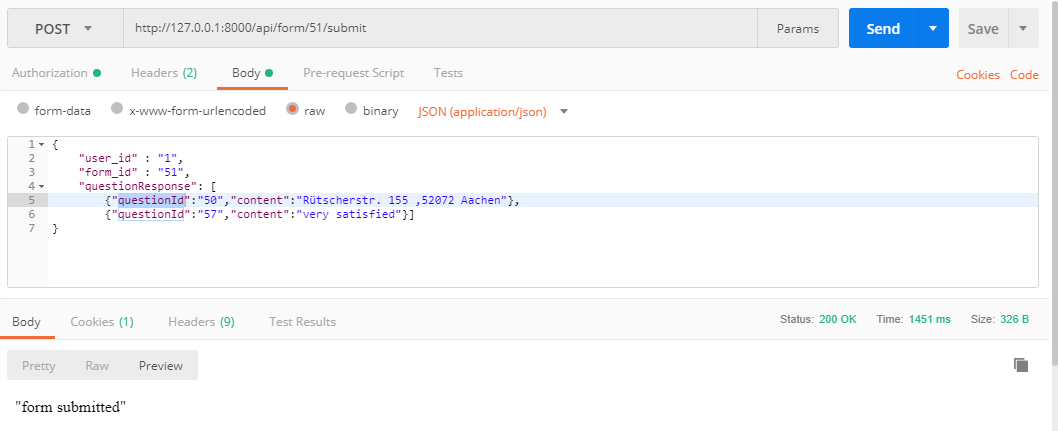
\includegraphics [width=16cm,height=7cm] {SprintImage/submitForm.PNG}
            \caption{Soumettre la réponse }
            \label{fig5}
        \end{center}
    \end{figure}

\section{Conclusion}
Nous avons réalisé au niveau de ce dernier chapitre, le choix de l’ensemble des composants logiciels combinés aux variantes techniques adoptées, ainsi que quelques artefacts de la gestion de projet.
        \clearpage
       
        
        \chapter*{Conclusion générale}
\addcontentsline{toc}{chapter}{Conclusion générale}
\markboth{Conclusion générale}{}

Dans le cadre de notre stage d'ingénieur, nous avons conçu et développé une application web pour la génération des formulaires dynamique sous forme d'un POC.\\

Afin d’atteindre nos objectifs, nous avons fait recours à la méthodologie Agile, pour assurer
la flexibilité et la bonne évolution de notre projet.

L’initiation de notre projet a été l’étape la plus complexe en termes du choix de la méthodologie la plus adaptée, de la maîtrise des langages de programmation, de l’analyse des
besoins et en terme de l’adaptation dans l’environnement de travail.

Néanmoins, nous avons pu surmonter plusieurs encombres et acquérir de nouvelles connaissances
en matière de méthodologie de travail, de nouvelle architecture, de technologie de
programmation web back-end avec Symfony et la maîtrise des services web de type REST.\\

Comme perspective, nous proposons de développer le reste de l'application tout en ajoutant les différentes types de champs ainsi un tableau de bord pour la visualisation des multiples réponses des utilisateurs.\\
Finalement, vu l’accomplissement du projet, nous souhaitons très fortement qu’il soit le fruit
du progrès, de l’évolution et qu’il reste à la hauteur des exigences de la société, nous souhaitons par ailleurs la satisfaction  de tous ses responsables.

        \clearpage
        
        % @author: 5misa
		% the command `\nocite{*}` is mandatory to avoid the “no \citation commands” error
        % https://tex.stackexchange.com/questions/18045/problem-with-compiling-bibtex-no-citation-commands-error
        %\nocite{*}
        \printbibliography[heading=bibintoc]
        
       % \chapter*{Annexes}
\addcontentsline{toc}{chapter}{Annexes}
\markboth{Annexes}{}
\stepcounter{chapter}
\addtocontents{lot}{\vspace{3.8mm}}
\addtocontents{lof}{\vspace{3.8mm}}

%Mettez vos annexes ici...

%===================== ANNEXE 1 =====================%
\section*{Annexe 1.~Exemple d'annexe}
\addcontentsline{toc}{section}{Annexe 1.~Exemple d'annexe}

Les chapitres doivent présenter l’essentiel du travail. Certaines informations-trop  détaillées  ou constituant un complément d’information pour toute personne qui désire mieux comprendre ou refaire une expérience décrite dans le document- peuvent être mises au niveau des annexes. Les annexes, {\bf placées après la bibliographie}, doivent donc être numérotées avec des titres (Annexe1, Annexe2, etc.).

\addcontentsline{lot}{table}{Annexe 1.1~~~Exemple tableau dans l'annexe}

Le tableau annexe 1.1 présente un exemple d'un tableau dans l'annexe.

{\raggedright \textbf{Tableau annexe 1.1:}~Exemple tableau dans l'annexe}
\begin{longtable}[c]{
    | p{.20\textwidth}
    | p{.50\textwidth} |
}
    \hline
        0 & 0 \\ \hline 
        1 & 1 \\ \hline 
        2 & 2 \\ \hline
        3 & 3 \\ \hline
        4 & 4 \\
    \hline

\end{longtable}

\newpage
%===================== ANNEXE 2 =====================%
\section*{Annexe 2.~Entreprise}
\addcontentsline{toc}{section}{Annexe 2.~Entreprise}

\addcontentsline{lof}{figure}{Annexe 2.1~~~Logo d'entreprise}

La figure annexe 2.1 présente le logo entreprise.
\begin{figure}[htpb]
    \centering
    \frame{\includegraphics[width=0.45\columnwidth]{Logo_Entreprise}}
    {\\\textbf{Figure annexe 2.1:} Logo d'entreprise}
\end{figure}

\end{document}